% Options for packages loaded elsewhere
\PassOptionsToPackage{unicode}{hyperref}
\PassOptionsToPackage{hyphens}{url}
%
\documentclass[
]{book}
\usepackage{amsmath,amssymb}
\usepackage{iftex}
\ifPDFTeX
  \usepackage[T1]{fontenc}
  \usepackage[utf8]{inputenc}
  \usepackage{textcomp} % provide euro and other symbols
\else % if luatex or xetex
  \usepackage{unicode-math} % this also loads fontspec
  \defaultfontfeatures{Scale=MatchLowercase}
  \defaultfontfeatures[\rmfamily]{Ligatures=TeX,Scale=1}
\fi
\usepackage{lmodern}
\ifPDFTeX\else
  % xetex/luatex font selection
\fi
% Use upquote if available, for straight quotes in verbatim environments
\IfFileExists{upquote.sty}{\usepackage{upquote}}{}
\IfFileExists{microtype.sty}{% use microtype if available
  \usepackage[]{microtype}
  \UseMicrotypeSet[protrusion]{basicmath} % disable protrusion for tt fonts
}{}
\makeatletter
\@ifundefined{KOMAClassName}{% if non-KOMA class
  \IfFileExists{parskip.sty}{%
    \usepackage{parskip}
  }{% else
    \setlength{\parindent}{0pt}
    \setlength{\parskip}{6pt plus 2pt minus 1pt}}
}{% if KOMA class
  \KOMAoptions{parskip=half}}
\makeatother
\usepackage{xcolor}
\usepackage{longtable,booktabs,array}
\usepackage{calc} % for calculating minipage widths
% Correct order of tables after \paragraph or \subparagraph
\usepackage{etoolbox}
\makeatletter
\patchcmd\longtable{\par}{\if@noskipsec\mbox{}\fi\par}{}{}
\makeatother
% Allow footnotes in longtable head/foot
\IfFileExists{footnotehyper.sty}{\usepackage{footnotehyper}}{\usepackage{footnote}}
\makesavenoteenv{longtable}
\usepackage{graphicx}
\makeatletter
\def\maxwidth{\ifdim\Gin@nat@width>\linewidth\linewidth\else\Gin@nat@width\fi}
\def\maxheight{\ifdim\Gin@nat@height>\textheight\textheight\else\Gin@nat@height\fi}
\makeatother
% Scale images if necessary, so that they will not overflow the page
% margins by default, and it is still possible to overwrite the defaults
% using explicit options in \includegraphics[width, height, ...]{}
\setkeys{Gin}{width=\maxwidth,height=\maxheight,keepaspectratio}
% Set default figure placement to htbp
\makeatletter
\def\fps@figure{htbp}
\makeatother
\setlength{\emergencystretch}{3em} % prevent overfull lines
\providecommand{\tightlist}{%
  \setlength{\itemsep}{0pt}\setlength{\parskip}{0pt}}
\setcounter{secnumdepth}{5}
\usepackage{booktabs}
\ifLuaTeX
  \usepackage{selnolig}  % disable illegal ligatures
\fi
\usepackage[]{natbib}
\bibliographystyle{plainnat}
\IfFileExists{bookmark.sty}{\usepackage{bookmark}}{\usepackage{hyperref}}
\IfFileExists{xurl.sty}{\usepackage{xurl}}{} % add URL line breaks if available
\urlstyle{same}
\hypersetup{
  pdftitle={L'opinione pubblica italiana e la guerra in Ucraina},
  pdfauthor={Pierangelo Isernia, Claudio Cozzi Fucile, Sergio Martini},
  hidelinks,
  pdfcreator={LaTeX via pandoc}}

\title{L'opinione pubblica italiana e la guerra in Ucraina}
\author{Pierangelo Isernia, Claudio Cozzi Fucile, Sergio Martini}
\date{2023-07-28}

\begin{document}
\maketitle

{
\setcounter{tocdepth}{1}
\tableofcontents
}
\hypertarget{lopinione-pubblica-italiana-e-la-guerra-in-ucrania}{%
\chapter*{L'opinione pubblica italiana e la guerra in Ucrania}\label{lopinione-pubblica-italiana-e-la-guerra-in-ucrania}}
\addcontentsline{toc}{chapter}{L'opinione pubblica italiana e la guerra in Ucrania}

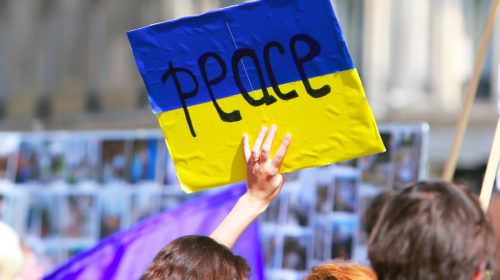
\includegraphics{Images/Ucrania.jpeg}

\hypertarget{introduzione}{%
\chapter{INTRODUZIONE}\label{introduzione}}

\hypertarget{la-guerra-e-lopinione-pubblica}{%
\section{La guerra e l'opinione pubblica}\label{la-guerra-e-lopinione-pubblica}}

La guerra in Ucraina rappresenta un evento senza precedenti nella storia postbellica europea, per almeno quattro ragioni. La prima è proprio il fatto di essere una ``guerra.''\footnote{Secondo una delle più citate definizioni operative di guerra interstatale (o intra-sistemica, da distinguersi da quelle extra-statali e civili), quella del \emph{Correlates of War}, è tale un conflitto che ha tre caratteristiche: è combattuto tra stati sovrani e riconosciuti dalla comunità internazionale come tali, vi siano almeno 1.000 morti in battaglia tra tutti gli stati coinvolti, e ciascun singolo partecipante soddisfi uno dei seguenti due requisiti: a) 100 morti in battaglia oppure b) un minimo di 1000 unità attive in combattimento nel teatro di guerra. Se poi la guerra dura più di un anno i morti in battaglia devono raggiungere una media annuale di 1000 casi (cf.~Singer e Small, 1982: 56; Sarkees, nd: 3).} In un'epoca in cui la frequenza delle guerre convenzionali è sensibilmente diminuita, a favore di altre forme di conflitto (Sarkees, Wayman e Singer, 2003), in particolare in Europa (e.g.~Gaddis, 1986) \footnote{Vi è un intenso dibattito sul fatto se le guerre interstatali siano effettivamente declinate (ad es. Pinker, 2011) o meno (ad es. Braumoeller, 2019). Per una discussione si veda Gleditsch (2013). Il \emph{Correlates of War Project} registra, nel periodo 1945-2007, una sola guerra interstatale -- come definita dal COW -- combattuta dalla Russia a fronte delle 40 che questo paese ha condotto tra gli inizi del '600 e il 1945.} la guerra ucraina rappresenta un tipico conflitto interstatale condotto con strumenti bellici convenzionali e secondo tattiche più vicine a quelle della Seconda Guerra Mondiale che a quelle tipiche delle guerre post-1945.

Una seconda novità è proprio il fatto che la guerra si svolga in Europa. Per la prima volta dalla fine della Guerra Fredda, una guerra convenzionale si combatte sul suolo del nostro continente. Durante la Guerra Fredda, le poche occasioni in cui i paesi europei, gli Stati Uniti e la Russia si sono fronteggiate in Europa con la minaccia del ricorso all'uso della forza non sono mai sfociate in un conflitto armato. Tipicamente, le guerre interstatali erano combattute in altre regioni del mondo, Inoltre, sono stati più spesso gli Stati Uniti ad essere invischiati in un conflitto (ad esempio in Corea e Vietnam), con i sovietici a sostenere la parte avversa.\footnote{La comparazione con l'Afghanistan è inappropriata, non solo perché non avviene in Europa, ma anche perché in quel caso l'intervento militare sovietico era diretto a sostenere un governo considerato amico, con gli americani che aiutavano invece gli avversari del regime afghano al potere (Litwak, 1992).}. In questo caso, invece, è la Russia ad essere impegnata in prima persona in una guerra interstatale contro l'Ucraina, sostenuta quest'ultima da Europa e Stati Uniti.

Una terza luogo novità è la \emph{coesione} della risposta dei paesi NATO all'attacco russo. Nel dopoguerra, raramente i paesi europei e gli Stati Uniti si sono trovati completamente \emph{eye-to-eye} quando si trattava di decidere che fare nei confronti alla Russia. A partire dalla guerra di Corea, con il timore del ricorso all'arma atomica da parte americana per fronteggiare la Cina, passando per la crisi degli Euromissili dei primi anni '80, gli europei si sono trovati spesso su posizioni dissonanti rispetto agli Stati Uniti nella valutazione della gravità della minaccia russa e nella scelta del modo migliore di fronteggiarla. In questo caso invece, almeno sinora, Stati Uniti e paesi europei hanno mostrato una sorprendente coesione nel sostenere l'Ucraina, economicamente e militarmente e nell'accettare i costi economici e politici di questa scelta.

È quindi stato abbastanza naturale, una volta compreso che la guerra sarebbe durata a lungo, che l'attenzione dei politici, degli osservatori e dei media si concentrasse sulle capacità di tenuta della coalizione occidentale. E per spiegare la tenuta di un paese democratico in guerra, l'enfasi si sposta, inevitabilmente, dai decisori politici ai cittadini, dagli eletti ai loro elettori, per saggiare la disponibilità dei secondi a sostenere un conflitto inaspettatamente più prolungato e gravoso di quanto originariamente previsto (Mueller, 1971; Aldrich et al, 2006). E, dal punto di vista della tenuta, l'Italia, tra tutti i grandi paesi europei che sostengono l'Ucraina, ha rappresentato per molti governi ed osservatori ad un tempo una sorpresa ed una fonte di preoccupazione.

La quarta ed ultima novità di questo conflitto riguarda infatti proprio \emph{l'Italia}. La determinazione con la quale il governo Draghi prima e quello Meloni dopo hanno appoggiato e dato concreto seguito alle determinazioni prese in sede NATO e UE, senza alcuna incertezza e con grande coerenza, ha ad un tempo sorpreso e preoccupato osservatori e alleati. La sorpresa nasce dal fatto che mentre l'Italia, negli ultimi anni, ha espresso nei confronti della Russia posizioni molto più simpatetiche del resto dei paesi europei, il governo Draghi si è invece immediatamente prodigato con risorse e dichiarazioni a sostegno dell'Ucraina \emph{whatever it takes}. La preoccupazione scaturiva dall'aspettativa, poi effettivamente realizzatasi, della vittoria della coalizione di centro-destra alle elezioni del settembre 2022. Tale coalizione, sin dall'inizio del conflitto russo-ucraino e ancor più durante la campagna elettorale, ha alimentato, con la crescente vocalità di alcuni dei suoi autorevoli leaders, perplessità e dubbi sulla posizione italiana nel conflitto e sulla sua capacità di perseguire con coerenza una politica di sostegno all'Ucraina. Perplessità e dubbi che, come vedremo, hanno trovato alimento in settori consistenti della nostra società civile e dell'opinione pubblica. Tuttavia, più di sei mesi dopo l'inizio della legislatura, il governo Meloni sembra continuare nel solco lasciato da Draghi. Ciò peraltro non ha significato un cambiamento radicale dell'opinione pubblica italiana e della sua posizione verso la guerra.

Per tutte queste ragioni, accertare cosa gli italiani pensino di questo conflitto e in che misura sostengano o si oppongano allo sforzo a favore del governo ucraino nella sua resistenza alla invasione russa, è un esercizio non solo utile scientificamente ma anche rilevante politicamente. Esso può contribuire infatti a fare chiarezza su molte impressioni e congetture circa le ragioni della scarsa disponibilità dell'opinione pubblica italiana a sostenere il ricorso all'uso della forza militare in quasi ogni circostanza possibile e per comprendere le condizioni in cui tale consenso venga meno o si rafforzi nel caso ucraino (Everts e Isernia, 2015).

\hypertarget{indagini-domande-e-comparazioni}{%
\section{Indagini, Domande e Comparazioni}\label{indagini-domande-e-comparazioni}}

Nel tentativo di offrire un quadro articolato e preciso della natura del sostegno (e della opposizione) italiana per la guerra in Ucraina, questo rapporto ricostruisce gli atteggiamenti dell'opinione pubblica italiana nei confronti di vari aspetti della guerra in Ucraina nel periodo compreso tra febbraio e giugno 2023. \footnote{Dal 24 febbraio alla fine di novembre 2022, il periodo coperto da questo rapporto, sono state condotte in Italia decine di indagini al cui interno sono state poste domande relative all'Ucraina. La \emph{Ukraine public opinion continuity guide} creata dal CIRCaP sull'Italia raccoglie più di 400 domande poste agli italiani su svariati aspetti della guerra e della sua evoluzione da febbraio a novembre 2022.} Il rapporto esamina gli atteggiamenti degli italiani su diversi temi, utilizzando tre ordini di comparazioni:

\begin{itemize}
\item
  nel tempo, coprendo il periodo tra lo scoppio del conflitto il 24 febbraio e giugno 2023;
\item
  nello spazio, rispetto ad altri paesi europei per i quali abbiamo dati disponibili e
\item
  tra formulazioni diverse delle stesse domande.
\end{itemize}

Per consentirci tale esame abbiamo raccolto tutte le domande rese disponibili sul sito \href{http://www.sondaggipoliticoelettorali.it/}{sondaggipoliticoelettorali.it} e da alcuni istituti di sondaggio (segnatamente IPSOS ed SWG con il bollettino settimanale Radar.\footnote{L'archivio è disponibile online sul sito del CIRCaP e del LAPS dell'Università di Siena.}

La convinzione su cui si fonda questo rapporto è infatti che, accanto alle analisi accurate delle determinanti individuali degli atteggiamenti, sia particolarmente utile una valutazione aggregata delle opinioni del pubblico su tematiche controverse come appunto quelle di politica estera. Guardare alla foresta delle domande disponibili, piuttosto che al singolo albero che di essa fa parte, consente da un lato un apprezzamento dell'effetto -- quando c'è -- del diverso modo di formulare le domande sugli atteggiamenti degli italiani e, dall'altro lato, consente di far emergere anche alcune interessanti caratteristiche del modo di sondare il pubblico da parte degli istituti di sondaggi italiani.

Come vedremo, la comparazione tra domande offerte con formulazioni diverse mostra l'importanza che il formato ed il contenuto delle domande hanno su tematiche complesse, caratterizzate da ampi margini di incertezza, nelle quali l'effetto di \emph{framing} esercvita una influenza nell'orientare le risposte degli intervistati. Il problema del c.d. \emph{question wording} lungi dall'essere un fattore di disturbo, una dimostrazione del fatto che con i sondaggi ``si può far dire di tutto alla gente,'' costituisce invece una fonte preziosa di informazioni, che aiuta a interpretare meglio cosa abbiano in mente gli intervistati quando rispondono ad una domanda e quali argomenti possono indurli a orientare le loro risposte in una direzione piuttosto che l'altra (citare qui Sudman, 19XX).

La sistematica raccolta di informazioni dice anche qualcosa sul modo in cui gli istituti di sondaggio affrontano temi pubblici attuali e prolungati, come appunto la guerra Ucraina. Tre ordini di considerazioni appaiono rilevanti a questo proposito. Una prima considerazione è la scarsa comparabilità delle formulazioni delle domande tra istituti diversi. Sebbene le domande sulla guerra in Ucraina siano numerose e coprano aspetti molto differenti, spesso di natura del tutto congiunturale (ad es. singoli eventi bellici, come Butcha), esse sono spesso formulate in maniera diversa e per questo difficilmente comparabili.

Una seconda osservazione è la scarsa attenzione prestata da molti istituti di sondaggio alla continuità delle domande nel tempo, un aspetto invece, quello dell'analisi delle tendenze dell'opinione pubblica a livello aggregato, particolarmente utile quando si tratta di analizzare un fenomeno che evolve nel tempo. I pochi trend disponibili sono stati realizzati soprattutto grazie a IPSOS e, in misura minore, a EMG, mentre molto più discontinua e \emph{ad hoc} è stata la produzione di dati da parte di altri istituti. Questa attenzione è scemata nel corso del tempo. Lo testimonia ad esempio il fatto che IPSOS, l'istituto che insieme a SWG e EMG, ha monitorato con più attenzione le opinioni degli italiani sul conflitto, ha dismesso il tracking sull'Ucraina dalla fine del 2022 e ora solo sporadicamente pone domande sul tema.

Infine, va segnalato come la guerra ucraina sia stata oggetto di una certa attenzione \emph{comparata}, con diverse indagini condotte contemporaneamente in più paesi, prevalentemente europei. Si segnalano qui in particolare le indagini eurobarometro (che ha inserito domande sull'Ucraina in diverse indagini nel corso del periodo coperto da questo rapporto) e quelle di SWG (Euroskopia) e YOUGOV. In questo campo sono stati però soprattutto i ricercatori a fornire le informazioni più sistematica, in particolare le rilevazioni EUOpinions e dello European University Institute.

Il rapporto è organizzato per aree tematiche. Esse sono:

\begin{itemize}
\item
  le preoccupazioni per la guerra e i suoi effetti, sia in assoluto che rispetto ad altre problematiche di politica interna;
\item
  le cause della guerra e le responsabilità per il suo scoppio, con riferimento anche alla percezione della Russia e di Putin;
\item
  gli effetti della guerra. Questa sezione si sofferma su tre ordini di temi:

  \begin{itemize}
  \tightlist
  \item
    le aspettative circa la sua durata e il suo possibile esito (chi vincerà?),
  \item
    il rischio di escalation militare (ad esempio con il possibile ricorso alle armi nucleari) e politica (ad es. con la estensione del conflitto ad altri paesi, segnatamente quelli della NATO;
  \item
    l'atteggiamento verso specifiche richieste da parte ucraina, come quella di una \emph{No-Fly-Zone} nel mese di marzo, o di armi pesanti a partire da aprile 2022.
  \end{itemize}
\item
  Il ruolo del nostro paese nel conflitto, con particolare riferimento sia alla decisione italiana di inviare armi, imporre sanzioni, aumentare le spese militari e, in via del tutto ipotetica, contribuire direttamente con le nostre truppe sia alle decisioni, multilaterali, relative ad una possibile accessione dell'Ucraina alla NATO e all'Unione Europea.
\item
  Gli effetti del conflitto, con particolare riferimento agli effetti economici delle sanzioni e quelli politici dei migranti.
\item
  La percezione del clima di opinione e degli atteggiamenti dei media da parte del pubblico italiano.
\end{itemize}

Ogni sezione è aperta da una breve sintesi dei risultati, seguita dalle tabelle rilevanti per ciascuna tematica. Ciascuna sezione discute prima alcuni aspetti metodologici relativi al modo in cui sono formulate le domande e ai loro effetti sulle distribuzioni delle risposte, seguite dalla descrizione degli atteggiamenti e della loro evoluzione nel tempo e, quando possibile, comparando le posizioni dell'opinione pubblica italiana a quella di altri paesi.

\hypertarget{preoccupazione-per-la-guerra}{%
\chapter{PREOCCUPAZIONE PER LA GUERRA}\label{preoccupazione-per-la-guerra}}

\hypertarget{formulazione-delle-domande}{%
\section{Formulazione delle domande}\label{formulazione-delle-domande}}

La misurazione delle preoccupazioni o priorità delle persone risente molto del contenuto e del formato delle domande che vengo poste. Quattro tipi di domande sono state utilizzate nel tempo in Italia per valutare l'importanza della guerra in Ucraina presso il pubblico italiano:

\begin{itemize}
\item
  \begin{enumerate}
  \def\labelenumi{\alph{enumi})}
  \tightlist
  \item
    Quelle che misurano la importanza/priorità di vari temi, le tipiche domande c.d. MIP (\emph{Most Important Problem}) o MII (\emph{Most Important Issues}). Sono incluse qui le domande che chiedono quali debbano essere le priorità per sé stessi (ad es. EB97.5), per il paese (ad es. EB97.5), per l'UE (ad es. EB98.1), per il Parlamento Europeo (ad es. EB97.3) e per il governo (es. Euromedia Research). Sono generalmente domande a risposte multiple (tra 2 e 3 possibili scelte). I temi non fanno riferimento esplicitamente all'Ucraina, ma a tematiche più generali, come la situazione internazionale.
  \end{enumerate}
\item
  \begin{enumerate}
  \def\labelenumi{\alph{enumi})}
  \setcounter{enumi}{1}
  \tightlist
  \item
    Quelle che esplicitamente e direttamente chiedono la preoccupazione per la guerra in Ucraina.
  \end{enumerate}
\item
  \begin{enumerate}
  \def\labelenumi{\alph{enumi})}
  \setcounter{enumi}{2}
  \tightlist
  \item
    Quelle che misurano la preoccupazione per le conseguenze della guerra (ad es. per la situazione economica o per il rischio di escalation sia geografica che di armamenti).
  \end{enumerate}
\item
  \begin{enumerate}
  \def\labelenumi{\alph{enumi})}
  \setcounter{enumi}{3}
  \tightlist
  \item
    Quelle che misurano i sentimenti e le emozioni prevalenti in questo periodo.
  \end{enumerate}
\end{itemize}

\hypertarget{principali-risultati}{%
\section{Principali risultati}\label{principali-risultati}}

\begin{itemize}
\tightlist
\item
  Quando si chiede agli intervistati se sono preoccupati della guerra in Ucraina, maggioranze schiaccianti (superiori all'80\%) rispondono positivamente.
\end{itemize}

Ai primi di marzo (Euromedia) l'88\% si dichiara molto o abbastanza preoccupato della guerra. Analoghe maggioranze trova Demos \& Pi/Demetra a marzo (93\%) e ad aprile (91\%). Percentuali simili ottiene SWG tra marzo e aprile 2022. I trend disponibili più lungo (quello EMG e quello IPSOS) rivelano una sostanziale stabilità nel tempo di questa preoccupazione. L'indagine IPSOS del 15-18 marzo 2022 riporta che l'86\% degli intervistati è molto o abbastanza preoccupato. Il 18-19 ottobre 2022 tale percentuale è all'80\%.

\begin{itemize}
\tightlist
\item
  Quando si chiede agli intervistati quali sono le loro preoccupazioni o priorità tra una lista lunga e variegata di temi, personali e pubblici, la percentuale di persone che seleziona l'Ucraina o le questioni internazionali è drasticamente minore. In questo caso, i problemi economici e quelli ambientali diventano più importanti di quelli legati all'Ucraina (ad es. Eurobarometro TTS e ASPEN).
\end{itemize}

Questo effetto è in parte determinato dal formato della domanda, nel senso che vincolati a scegliere tra temi molto diversi, gli intervistati prioritizzano quelli che per loro sono i più rilevanti personalmente. Lasciati liberi di indicare il loro livello di preoccupazione per qualsiasi problema, risponderebbero di esserlo in numero molto maggiore. Un esempio di questo effetto si trova comparando le risposte a diversi formati di una domanda simile, che chiede la preoccupazione per la situazione internazionale rispetto alla guerra ai confini dell'Europa in due formati diversi. Il primo formato invita a scegliere tre problemi tra più di 10, la seconda chiede invece, per ogni problema, quanto preoccupato è l'intervistato. Nel giugno-luglio (EB97.5) il 12\% degli italiani menzionano la situazione internazionale come uno dei due temi più importante per loro personalmente, dovendo scegliere tra molti, mentre il 58\% risponde che la guerra nelle vicinanze dell'UE è molto importante quando invitati ad indicare se, per loro, questa issue è importante.

\begin{itemize}
\tightlist
\item
  In entrambi i tipi di formulazione, la preoccupazione per la guerra è leggermente calata nel tempo (trends IPSOS ed EMG).
\end{itemize}

I trends EMG e IPSOS rivelano un andamento simile, con circa l'80\% degli intervistati che si dichiarano preoccupati della guerra e della sua evoluzione, ma si ravvisa una leggera tendenza al calo del numero di persone preoccupate, nel caso della serie EMG a partire da aprile (con una leggera risalita a maggio) e nel caso IPSOS tra aprile e maggio con una ulteriore caduta a luglio e una ripresa dopo il mese di agosto. Il trend SWG non mostra questo calo perché si interrompe prima, finendo ad aprile.

\begin{itemize}
\item
  Richiesti di spiegare quali sono le fonti della preoccupazione per la guerra, l'attenzione è soprattutto per le conseguenze economiche della guerra, piuttosto che per quelle politiche, militari o personali (IPSOS).
\item
  • Invitati a segnalare quali sono le ragioni o gli aspetti della guerra che preoccupano di più, quelli economici emergono come prevalenti, anche se la distribuzione è fortemente influenzata dal tipo di conseguenze indicate e dalla possibilità di sceglierne più d'una o solo una.
\end{itemize}

La domanda che più direttamente consente di comparare quali conseguenze della guerra sono più preoccupanti è quella IPSOS che chiede l'aspetto più preoccupante, di natura economica, politica e umanitaria. Le conseguenze economiche sono sempre menzionate da una maggioranza relativa, seguita da un terzo a un quarto di intervistati che menziona quelle belliche e da un decimo che riporta quelle umanitarie. Queste priorità sono confermate dalla domanda SWG nella quale il numero di persone preoccupate che ``il quadro economico peggiori pesantemente passa dal 51\% del 9 marzo al l'86\% del 23 marzo. Le vittime, l'uso dell'arma nucleare e la possibilità che dopo l'Ucraina, la Russia invada altri paesi totalizzano percentuali nettamente inferiori. In alcune indagini dei primi due mesi, tuttavia, le preoccupazioni sul conflitto appaiono prevalenti rispetto a quelle economiche. Questo avviene \emph{prima} dello scoppio del conflitto (ad es. l'indagine SWG del 16-18 febbraio) o in isolati indagini nei primi mesi (ad es. l'indagine Euromedia, 27-28 aprile).

\begin{itemize}
\tightlist
\item
  Tra gli aspetti economici che suscitano preoccupazione, vi sono l'aumento dei prezzi (indagini EMG), anche se la maggioranza l'attribuisce agli speculatori piuttosto che alla guerra (IPSOS, 14 marzo). La maggioranza teme gli effetti sulla propria personale situazione economica (Noto sondaggi) o addirittura già ne sente gli effetti ad aprile (Noto sondaggi).
\end{itemize}

\href{https://github.com/LucianaFazio/Ucrania/blob/main/PDF_Appendice/II\%20Preoccupazioni\%20Ucraina\%20v.6.pdf}{Appendice}

\hypertarget{le-cause-della-guerra-di-chi-uxe8-la-colpa-blaming}{%
\chapter{LE CAUSE DELLA GUERRA: DI CHI È LA COLPA (BLAMING)}\label{le-cause-della-guerra-di-chi-uxe8-la-colpa-blaming}}

\hypertarget{formulazione-delle-domande-1}{%
\section{Formulazione delle domande}\label{formulazione-delle-domande-1}}

L'esame delle cause della guerra nell'opinione degli intervistati è stato condotto da molteplici punti di vista. Possiamo classificare le domande poste su questi temi sulla base di tre aspetti.

\begin{itemize}
\item
  \begin{enumerate}
  \def\labelenumi{\alph{enumi})}
  \tightlist
  \item
    Il primo è il contenuto della domanda. Alcune domande cercano di accertare le responsabilità della guerra, di chi è insomma la colpa (il c.d. \emph{blaming}) mentre altre esplorano le motivazioni o cause della guerra. Rilevano qui le opinioni degli intervistati sulle responsabilità rispettive dei due schieramenti circa l'inizio e la persistenza della guerra, nonché quelle che approfondiscono le motivazioni o cause prevalenti del conflitto.
  \end{enumerate}
\item
  \begin{enumerate}
  \def\labelenumi{\alph{enumi})}
  \setcounter{enumi}{1}
  \tightlist
  \item
    Un secondo aspetto attiene al formato della domanda. Fondamentalmente è possibile distinguere due tipi di formati delle domande che esplorano questi temi. Da un lato, vi sono domande che chiedono direttamente di indicare di chi è la colpa o la responsabilità del conflitto tra le due parti. Dall'altro vi sono domande che invece elencano o suggeriscono una serie di motivazioni e/o spiegazioni possibili della guerra. Non sorprendentemente, i due tipi di domande producono risultati sensibilmente diversi.
  \end{enumerate}
\item
  \begin{enumerate}
  \def\labelenumi{\alph{enumi})}
  \setcounter{enumi}{2}
  \tightlist
  \item
    Infine, un terzo aspetto è quello della comparabilità delle domande nel tempo o nello spazio. Gran parte delle domande sono state poste solo occasionalmente dai vari istituti di sondaggio, rendendo quindi difficile una valutazione dell'andamento dei giudizi degli italiani nel tempo, con una sola eccezione, quella di IPSOS sulle cause del conflitto, che è stata reiterata per diversi mesi. Vi è anche un caso in cui la domanda sulla responsabilità è stata posta in diversi paesi, consentendo una valutazione della posizione italiana con quella di altri paesi.
  \end{enumerate}
\end{itemize}

\hypertarget{principali-risultati-1}{%
\section{Principali risultati}\label{principali-risultati-1}}

\begin{itemize}
\tightlist
\item
  Quando si chiede agli intervistati di indicare chi è il principale responsabile del conflitto, maggioranze sostanziali di circa due terzi degli intervistati indicano nella Russia il responsabile principale.
\end{itemize}

Diverse domande hanno esplorato il tema delle responsabilità della guerra. Tra febbraio e marzo 2022 circa l'80\% degli intervistati SWG ritiene l'attacco della Russia all'Ucraina ``inaccettabile, da condannare severamente'' e il 71\% degli intervistati SWG del 21-25 marzo esprime una ``condanna totale dell'attacco.'' Similmente tra marzo e aprile 2022 il 77\% degli intervistati da Demetra considera l'attacco grave e ingiustificato.

Il \emph{wording} della domanda sembra avere un leggero effetto sulle rispose. Quando la domanda usa termini più neutrali rispetto a ``colpa'' e ``condanna'', parlando ad esempio di ``motivazioni'' (ad es. Euromedia ed EMG) o di ``ragioni,'' le percentuali di intervistati che puntano il dito sulla Russia restano elevate, ma sono leggermente inferiori a quelle appena citate. Ad esempio, la percentuale di intervistati che ritiene prevalenti le motivazioni (o le ragioni) ucraine scende al 57\%-60\% in una serie di domande EMG.

\begin{itemize}
\tightlist
\item
  Quando la domanda sollecita la risposta ad una più articolata serie di motivazioni, il giudizio degli italiani si fa più sfumato e meno netta emerge la responsabilità esclusiva della Russia.
\end{itemize}

Nel periodo compreso tra il 23 e il 28 marzo Termometro Politico ed EMG hanno posto due domande più articolate di quelle esaminate sinora, elencando tra le alternative di risposta considerazioni diverse. Ad esempio, Termometro politico nell'invitare a dare un giudizio sull'intervento militare della Russia in Ucraina offriva la scelta tra la seguente serie di motivazioni: ``È stato un atto molto grave, una prevaricazione intollerabile verso uno stato sovrano;'' ``È stato un atto avventato e sbagliato, secondo me, ma se rimane limitato al Donbass non è così grave;'' ``È stata una mossa comprensibile, se rimane limitata al Donbass, si è trattato di un giusto atto di protezione verso la minoranza russa;'' e ``Ha fatto bene, l'Ucraina rischia di diventare un fantoccio occidentale, dovrebbe tornare sotto l'egida di Mosca.'' Non sorprendentemente, l'opportunità di offrire un giudizio più articolato riduce al 39\% la percentuale di intervistati che condanna recisamente l'intervento militare come ``atto molto grave.'' Il resto degli italiani aderisce a giudizi più sfumati, con un 14\% dei quali è decisamente apologetico nei confronti della Russia, approvandone l'operato. L'indagine EMG del 28 marzo pone all'intervistato delle alternative di ancor più ampia portata e anche qui non più del 20\% aderisce ad una posizione di condanna decisa dell'operato russo, sottoscrivendo che ``È una guerra tra due Paesi, in cui uno ha illegittimamente aggredito l'altro.'' Il resto degli intervistati preferisce ascrivere il conflitto ad uno scontro di più ampia portata. Infine, la domanda IPSOS sulle cause della guerra -- che riprende la nota tesi avanzata dai neorealisti circa le responsabilità della NATO nell'aver determinato le reazioni russe -- offre anch'essa una serie più articolata di ragioni della guerra, quali ``La minaccia della NATO giustifica l'invasione Russa dell'Ucraina;'' ``La Nato minaccia la Russia, ma ciò non giustifica l'invasione;'' e ``La Russia ha solo cercato un pretesto e non ha giustificazioni per l'invasione dell'Ucraina.'' E anche in questo caso aderiscono alla tesi della responsabilità esclusiva della guerra percentuali mai molto superiori al 50\% di intervistati.

\begin{itemize}
\tightlist
\item
  Nel corso dei mesi la percentuale di italiani che tendono ad attribuire la colpa della guerra alla Russia cala leggermente mentre aumenta quella di coloro che non rispondono.
\end{itemize}

Una prima, ancorché circoscritta, serie temporale è quella Euromedia Research ed EMG tra marzo e maggio che evidenzia come il fronte di coloro che ritengano prevalenti le motivazioni ucraine cresca leggermente nel tempo (dal 57\% di marzo al 61\% di maggio). La più lunga serie temporale IPSOS sulle ``cause del conflitto'' mostra un leggero declino di coloro che ritengono che ``La Russia ha solo cercato un pretesto e non ha giustificazioni per l'invasione dell'Ucraina.'' La domanda in direzione di una maggiore incertezza cica l'attribuzione delle colpe. A marzo (28-30 marzo) la percentuale di coloro che ritrovavano nella Russia la responsabile unica del conflitto erano il 49\%, mentre un altro 28\% riteneva che la NATO minacciasse la Russia ma che ciò non giustificasse l'invasione, e un residuo 6\% era composto da coloro che ritrovavano invece nella minaccia della NATO una giustificazione dell'invasione. A settembre il fronte di coloro che ritrovavano nella Russia l'unica responsabile è sceso al 42\%, mentre è cresciuto dal 17\% al 25\% la percentuale di coloro che non sanno o non rispondono.

\begin{itemize}
\tightlist
\item
  L'Italia si conferma tra i paesi nei quali le percentuali di persone che tendono ad attribuire le colpe alla Russia sono sistematicamente inferiori -- anche se di poco -- a quelle della gran parte dei paesi europei e sempre minori di Francia, Germania, Inghilterra e Spagna.
\end{itemize}

Tra l'8 e l'11 marzo 2022 SWG-Euroskopia ha chiesto ai cittadini di 6 paesi europei se l'attacco russo all'Ucraina fosse inaccettabile, inaccettabile ma comprensibile o accettabile. L'Italia è al penultimo posto (seguita solo dalla Grecia) con il 71\% che lo ritiene inaccettabile (a fronte del 60\% dei greci) e il 19\% inaccettabile ma comprensibile. Questa percentuale è inferiore a quella di Olanda (88\% inaccettabile), Spagna (86\%), Germania (82\%) e Francia (78\%). Alla domanda ``Le autorità russe sono le principali responsabili della situazione attuale'' posta nel Flash Eurobarometro 506 del 14-20 aprile 2022 il 73\% degli italiani hanno risposto di essere d'accordo. Questo pone gli italiani al 18° posto, dopo tutti i principali paesi europei occidentali e al di sotto della media europea del 78\%.

\begin{itemize}
\tightlist
\item
  Quando si chiede agli intervistati di giudicare l'attacco della Russia all'Ucraina solide maggioranze assolute si trovano d'accordo sulla condanna totale o parziale dell'attacco, quando però si interrogano le posizioni degli intervistati o la risposta dell'Ucraina nel corso dei mesi le maggioranze solide in favore di quest'ultima tendono a consumarsi.
\end{itemize}

Nel sondaggio SWG del 23-25 marzo si osserva che l'82\% degli intervistati condanna l'attacco nei confronti dell'Ucraina (71\% totalmente e l'11\% parzialmente), in linea con le rilevazioni SWG del 25-28 Febbraio e del 23-28 marzo dove, sullo stesso numero di intervistati (800), il 79\% in ambedue i rilevamenti ritiene che l'attacco sia inaccettabile e da condannare severamente, e in linea altresì -- anche se leggermente in calo -- con i dati di Demetra dell'11-12 aprile sulla scelta della Russia di iniziare l'intervento militare il 76\% la ritiene grave e ingiustificata. Valutando invece gli schieramenti degli intervistati si osserva che solo il 58\% di questi si dichiara apertamente con l'Ucraina (EMG 16 aprile), solo il 64\% spera che Putin perda la guerra mentre il 26\% sono indecisi (SWG 27 aprile-2 maggio), infine, ad ottobre (Euromedia Research 26 ottobre), soltanto il 36\% riteneva ancora che l'Ucraina dovesse resistere a tutti i costi, la maggioranza (quasi assoluta) si schierava su posizioni di concessioni alla Russia (49\%).

\href{https://github.com/LucianaFazio/Ucrania/blob/main/PDF_Appendice/III.\%20Le\%20cause\%20della\%20guerra_v.5.pdf}{Appendice}

\hypertarget{landamento-della-guerra-come-finiruxe0}{%
\chapter{L'ANDAMENTO DELLA GUERRA: COME FINIRÀ?}\label{landamento-della-guerra-come-finiruxe0}}

\hypertarget{formulazione-delle-domande-2}{%
\section{Formulazione delle domande}\label{formulazione-delle-domande-2}}

L'esame dell'andamento guerra nell'opinione degli intervistati è stato condotto da molteplici punti di vista. Possiamo distinguere le domande rivolte agli intervistati su questi temi prevalentemente sulla base del contenuto della domanda e, all'interno di classi divise per contenuto, è possibile altresì distinguere le domande in funzione del formato dell'indagine

\begin{itemize}
\item
  \begin{enumerate}
  \def\labelenumi{\alph{enumi})}
  \tightlist
  \item
    Il contenuto della domanda diversifica sensibilmente i sondaggi tra di loro. Alcune domande cercano di accertare il vincitore attuale e futuro del conflitto, mentre altre domande indagano i pericoli avvertiti dagli intervistati circa possibili escalation, ovvero le considerazioni circa la durata effettiva della guerra o, ancora le condizioni per porvi fine.
  \end{enumerate}
\item
  \begin{enumerate}
  \def\labelenumi{\alph{enumi})}
  \setcounter{enumi}{1}
  \tightlist
  \item
    Un secondo aspetto attiene al formato della domanda e ciò rileva particolarmente all'interno di ogni classe divisa per contenuto. Ad esempio, nel primo paragrafo che indaga i vincitori attuali e presunti futuri, si osservano differenze significative a seconda di come la domanda venga posta, ciò è vero anche nel secondo paragrafo circa le preoccupazioni di escalation: Il \emph{wording} nel sondaggio sembra avere un effetto sulle risposte.
  \end{enumerate}
\item
  \begin{enumerate}
  \def\labelenumi{\alph{enumi})}
  \setcounter{enumi}{2}
  \tightlist
  \item
    Infine, un terzo aspetto è quello della comparabilità delle domande nel tempo. Sebbene la maggior parte delle domande siano state poste solo \emph{una tantum} dai vari istituti di sondaggio -- il che complica un'eventuale analisi dell'andamento dell'opinione pubblica degli italiani nel tempo -- si ritrovano, soprattutto circa il vincitore del conflitto, serie continuative nel tempo.
  \end{enumerate}
\end{itemize}

\hypertarget{principali-risultati-2}{%
\section{Principali risultati}\label{principali-risultati-2}}

\hypertarget{esito-del-conflitto-chi-vinceruxe0}{%
\subsection{Esito del conflitto: chi vincerà?}\label{esito-del-conflitto-chi-vinceruxe0}}

\begin{itemize}
\tightlist
\item
  Quando si chiede contemporaneamente agli intervistati chi stia attualmente vincendo la guerra e chi si pensa che vincerà il conflitto, si ottengono risultati sensibilmente diversi
\end{itemize}

Diverse domande hanno esplorato il tema del vincitore -- presunto e attuale -- del conflitto in corso. Ad Aprile 2022 il 22\% degli intervistati di Noto Sondaggi ritiene che la Russia di Putin stia attualmente vincendo il conflitto e il 26\% degli intervistati, sempre di Noto Sondaggi, conferma anche che la Russia vincerà la guerra. La medesima valutazione non può essere fatta però per il fronte ucraino: il 47\% degli intervistati crede che l'Ucraina stia attualmente vincendo, ma soltanto il 28\% crede che vincerà. Logicamente, si osservano variazioni importanti anche nel gruppo degli indecisi: coloro che non sanno chi, tra Russia e Ucraina, stia vincendo momentaneamente il conflitto sono circa il 30\%, chi invece non sa esprimersi su chi vincerà il conflitto sono quasi il 50\%.
Questa valutazione può essere riproposta per Maggio nei sondaggi Ipsos, EMG, Demopolis. Rimane stabile la percentuale di coloro che credono che la Russia stia vincendo (23\%) ma diminuisce il numero di coloro che credono che Putin vincerà la guerra (12\%). Si osserva poi che la percentuale degli intervistati che ritengono l'Ucraina vincente nel momento in cui viene posta la domanda è sempre maggiore rispetto alla percentuale di chi ritiene che l'Ucraina vincerà la guerra (47\%--28\% ad Aprile, 28\%--20\% a Maggio).

\begin{itemize}
\tightlist
\item
  Quando si chiede agli intervistati chi vincerà la guerra si osserva che, nel tempo, diminuiscono coloro che ritenevano la Russia di Putin vincitrice del conflitto, ma contemporaneamente ad aumentare non è il fronte di chi crede che sarà l'Ucraina di Zelensky a vincere, bensì quello degli indecisi che non sanno o preferiscono non indicare.
\end{itemize}

A Marzo 2022 il 52\% degli intervistati per il Termometro politico sosteneva che la Russia di Putin avrebbe vinto la guerra (sebbene il 24\% di questi ritenevano altresì che all'occupazione russa l'Ucraina avrebbe resistito duramente), il 37\% riteneva invece che sarebbe stata l'Ucraina a vincere e solo il 10\% preferiva non rispondere o non sapeva. Sempre a Marzo: per il 58\% degli intervistati Ipsos la Russia avrebbe vinto la guerra, solamente per il 13\% a vincere sarebbe stata l'Ucraina, mentre il numero di coloro che non sapevano o non volevano esprimersi si attestava intorno al 20\%.
Ad Aprile, secondo Noto Sondaggi, il fronte di coloro che ritenevano che la Russia avrebbe vinto la guerra si assottiglia al 26\%, similmente anche il numero di coloro che ritenevano il fronte ucraino come prossimo vincitore si attesta attorno a percentuali simili (28\%), a crescere sensibilmente, invece, è il gruppo di chi non sa o non vuole indicare un netto vincitore: il 46\% degli intervistati, infatti, preferisce non esprimersi.
Si osservi, infine, che a Maggio (IPSOS) il numero di coloro che ritenevano la Russia come futura vincitrice del conflitto crolla al 12\%, similmente, anche chi riteneva l'Ucraina vincitrice scende al 20\%, la terza opzione è preferita dal 68\% degli intervistati e, di questi, il 12\% non sa o non vuole indicare, ma il 56\% indica ``nessuno'' come futuro vincitore.

\begin{itemize}
\tightlist
\item
  Quando si chiede agli intervistati chi nel momento in cui la domanda viene posta stia vincendo la guerra, maggioranze decrescenti nel tempo si schierano sul lato russo e sul lato ucraino, aumenta consequenzialmente e progressivamente il numero degli indecisi.
\end{itemize}

A Marzo 2022 nel momento in cui la domanda gli era rivolta il 28\% degli intervistati Ipsos credeva che la Russia stesse vincendo la guerra, mentre il 39\% riteneva che l'Ucraina fosse in vantaggio e soltanto il 33\% non sapeva o non voleva indicare un vincitore.
A Maggio alla stessa domanda il 23\% degli intervistati EMG indicava la Russia di Putin come forza militarmente in vantaggio sull'altro schieramento, subendo nel corso di due mesi una perdita in termini percentuali di 5 punti. Una riduzione più significativa si registrava invece sull'altro lato dello schieramento: solo il 28\% riteneva l'Ucraina di Zelensky in vantaggio, facendo rilevare un calo in termini percentuali di 11 punti rispetto ai precedenti 39. Se ne trae che l'unica opzione che ha visto crescere le proprie percentuali sia la terza: chi non sapeva o non voleva esporsi passa dal 33\% al 49\% (+16\%). Nel giro di due mesi quasi un intervistato su due non sapeva o non voleva indicare quale schieramento stesse vincendo il conflitto nel momento in cui la domanda gli veniva posta.

\begin{itemize}
\tightlist
\item
  Quando si chiede agli intervistati come terminerà la guerra, maggioranze progressivamente crescenti nel tempo prevedono la conclusione del conflitto mediante il ricorso a una soluzione diplomatica o comunque con un compromesso tra le parti.
\end{itemize}

Dalla serie EMG svoltasi a Maggio si evince che maggioranze crescenti prospettano il ricorso a un compromesso tra le parti. Se a metà Maggio il 44\% degli intervistati EMG prevede il ricorso a una soluzione diplomatica per porre fine al conflitto bellico, alla fine di Maggio il 57\% degli intervistati si augura un compromesso che possa mettere d'accordo i diversi schieramenti. È interessante osservare come, allo stesso tempo, a decrescere non sia il numero di coloro che sostengono convintamente la vittoria militare e schiacciante di uno dei due schieramenti -- Russo o Ucraino che sia--, bensì il fronte degli indecisi: il 17-19 Maggio il 42\% degli intervistati EMG preferivano non rispondere alla domanda, a fine maggio la stessa opzione è scelta solamente dal 24\% degli intervistati. Si rinforza anche se in misura ridotta e dopo un breve e leggero declino, all'opposto, il fronte di chi crede che la guerra si concluderà con la vittoria di una delle due parti.

\hypertarget{escalation}{%
\subsection{Escalation}\label{escalation}}

\hypertarget{escalation-rischio-guerra-nucleare}{%
\subsubsection{\texorpdfstring{\emph{Escalation: Rischio guerra nucleare}}{Escalation: Rischio guerra nucleare}}\label{escalation-rischio-guerra-nucleare}}

\begin{itemize}
\tightlist
\item
  Quando si chiede agli intervistati se vi sia un rischio di una escalation nucleare, si osservano preoccupazioni decrescenti nel tempo e differenze significative nell'eventualità in cui venga nominata direttamente l'espressione \emph{``guerra atomica''}.
\end{itemize}

Diverse domande hanno esplorato il tema dell'eventualità di una escalation nucleare. A Marzo 2022 il 72\% degli intervistati Euromedia Research ritiene che la possibilità di una escalation nucleare sia avverabile, similmente ad Aprile, il 68\% degli intervistati della serie EMG (5 sondaggi ripetuti nell'arco di due mesi) temevano che la guerra potesse degenerare in un conflitto nucleare, a Maggio la stessa percentuale si riduce attestandosi intorno al 60\%.

La serie continuata IPSOS conferma e rafforza quanto detto: a Marzo il 31\% degli intervistati ritenevano probabile (molto e abbastanza) il ricorso ad armi nucleari, a Settembre lo stesso fronte era invece formato dal 19\% del campione. Contemporaneamente, se a Marzo il 45\% degli intervistati ritenevano poco o per nulla probabile un conflitto nucleare, a Settembre gli stessi pesavano per il 56\% nel campione analizzato.
Si osservi però come ad Ottobre, e solo da Ottobre, la preoccupazione per un conflitto nucleare ritorni nuovamente predominante nell'opinione pubblica: il 30\% degli intervistati l'11 e il 12 Ottobre dichiarano molto o abbastanza probabile un ricorso ad armi nucleari (valori identici a quelli di Marzo), allo stesso tempo anche il fronte di chi crede poco o per nulla probabile un conflitto nucleare ritorna ai valori di Marzo attestandosi attorno al 40\% degli intervistati

Il \emph{wording} nel sondaggio sembra avere un effetto sulle risposte: quando una domanda usa il termine ``bomba atomica'', ovvero ``guerra atomica'', vocaboli meno neutrali rispetto a ``conflitto nucleare'', le percentuali di intervistati che si dimostrano preoccupati di un eventuale escalation si riduce di molto: ad Aprile il 34\% e ad Ottobre il 43\% degli intervistati del Termometro Politico ritengono probabile o possibile una guerra nucleare.

\hypertarget{escalation-terza-guerra-mondiale-e-no-fly-zone}{%
\subsubsection{\texorpdfstring{\emph{Escalation: Terza guerra mondiale e No fly zone}}{Escalation: Terza guerra mondiale e No fly zone}}\label{escalation-terza-guerra-mondiale-e-no-fly-zone}}

\begin{itemize}
\tightlist
\item
  Quando si chiede agli intervistati se vi sia un rischio di una escalation su scala mondiale del conflitto, si osservano preoccupazioni decrescenti nel tempo: maggioranze gradualmente più consistenti si convincono che il conflitto rimarrà nei confini dei due paesi.
\end{itemize}

A Marzo 2022 solo il 29\% degli intervistati IPSOS ritiene che il conflitto non travalicherà i confini dei due paesi coinvolti, ad Aprile circa il 40\% degli intervistati DemosPi \& Demetra e EMG si confermano convinti che il conflitto non coinvolgerà nessun altro paese al di fuori di Ucraina e Russia.
Si segnala altresì che inserendo nell'analisi un'ulteriore variabile si ottengono risultati sensibilmente diversi: nell'eventualità di una \emph{no fly zone} a Marzo per l'83\% degli intervistati Demopolis si correrebbe il pericolo di un coinvolgimento della guerra su scala mondiale.

Questo trend è confermato dalla serie continuata IPSOS che da marzo ad Ottobre indaga l'opinione pubblica circa i rischi di una degenerazione del conflitto : se a Marzo 2022 il 24\% degli intervistati ritiene plausibile che il conflitto russo-ucraino degeneri in una guerra mondiale, a Settembre la stessa opinione è condivisa solo dall'11\% della popolazione.
Parimenti: a Marzo 2022 il 26\% degli intervistati ritiene che il conflitto rimarrà confinato nei confini dei due paesi belligeranti, a Settembre la stessa posizione è sostenuta da ben il 39\% degli intervistati. Si consideri, infine, che come per il paragrafo precedente ad Ottobre si osservano valori contrastanti con i trend registrati durante i 9 mesi precedenti: le percentuali delle rispettive posizioni aumentano e diminuiscono ritornando (ovvero, riavvicinandosi) alle stime di Marzo: solo il 26\% degli intervistati il 5-6 Ottobre ritiene che il conflitto resterà isolato nei confini dei due paesi in guerra; il 20\% degli intervistati l'11 e il 12 Ottobre ritengono invece di nuovo plausibile un conflitto su scala mondiale.

\hypertarget{a-quali-condizioni-finire-il-conflitto-e-possibilituxe0-di-negoziati}{%
\subsection{A quali condizioni finire il conflitto e possibilità di negoziati}\label{a-quali-condizioni-finire-il-conflitto-e-possibilituxe0-di-negoziati}}

\begin{itemize}
\tightlist
\item
  Quando si chiede agli intervistati le condizioni con cui finire il conflitto, maggioranze solide nel tempo ritengono che l'Ucraina debba fare delle concessioni alla Russia e il compromesso rimane costantemente l'opzione favorita.
\end{itemize}

Molteplici domande indagano l'opinione degli intervistati circa le condizioni con cui porre termine alla guerra in corso. Resta costante la percentuale di coloro che, nel corso del tempo e a domanda diretta, rispondono che l'unico metodo per concludere il conflitto sia la resa dell'Ucraina nei confronti della Russia. Il 38\% degli intervistati Euromedia Research a Marzo ritiene che l'Ucraina debba arrendersi (nonostante il 76\% degli intervistati Noto Sondaggi dello stesso mese ritengano che la maggiore responsabilità sia proprio della Russia), il 43\% degli intervistati Ipsos a Marzo condivide questa opinione, il 52\% degli intervistati SWG a Maggio crede che il conflitto si possa concludere o con la sconfitta totale Ucraina (6\%) o con il controllo dei territori occupati dalla Russia (46\%). Addirittura, il 74\% degli intervistati del Termometro Politica di Maggio ritengono che sarebbe accettabile un accordo di pace che includesse l'annessione da parte della Russia di tutto o parte del territorio ucraino occupato.

Proprio il tema della cessione di territori ucraini alla Russia incontra nel tempo percentuali significative, prossime alla maggiorana relativa: solo il 10\% del campione di SWG di Aprile dichiara che l'Ucraina non debba concedere nulla alla Russia, il 40\% dei soggetti ascoltati dal Proger IndexResearch a Maggio credono che l'Ucraina debba accettare una qualche forma di rinuncia territoriale (il 37\% è contrario il 23\% non sa o non indica), il 46\% degli intervistati dal Termometro Politico di Giugno ritengono che non costituisca un precedente pericoloso la cessione di territori occupati, il 49\% del campione di Euromedia Research ad Ottobre crede che l'Ucraina debba fare delle concessioni per accelerare il processo di pace.

Allo stesso tempo maggioranze rilevanti si augurano un compromesso tra le parti al fine di porre termine, nel minor tempo possibile, al conflitto in atto. Ad Aprile il 56\% degli intervistati di Euromedia Research credono che il compromesso tra le parti sia l'obiettivo sul quale puntare, sempre ad Aprile il 55\% del campione di EMG dichiara che l'Europa dovrebbe in tutti modi promuovere la trattiva diplomatica, la stessa opzione è favorita dal 62\% degli intervistati Ipsos a Maggio, sempre a Maggio il 62\% degli intervistati EMG credono che una soluzione diplomatica sia possibile (in tempi lunghi e in tempi brevi), infine, anche ad Ottobre il 54\% del campione ascoltato dal Proger IndexResearch auspicano un compromesso mediato tra Putin e le forze politico -- istituzionali dell'Occidente.

\hypertarget{durata-conflitto}{%
\subsection{Durata conflitto}\label{durata-conflitto}}

\begin{itemize}
\tightlist
\item
  Quando si chiede agli intervistati una stima della durata del conflitto, salvo un primo momento, si osserva una certa stabilità nella distribuzione delle preferenze, con effetti interessanti dovuti al numero di opzioni a disposizione da parte degli intervistati.
\end{itemize}

A Marzo il 21\% degli intervistati EMG riteneva che il conflitto si sarebbe concluso nel giro di poche settimane, a Maggio la percentuale subisce un significativo contraccolpo riducendosi a cifre sempre inferiori al 10\% degli intervistati, fino a toccare la percentuale minima nel sondaggio del 12 Maggio: 3\%.

È utile osservare altresì come, nell'eventualità in cui agli intervistati siano date più opzioni di scelta la percentuale di coloro che non sa o non si vuole esprimere sia sensibilmente contenuta: sondaggio dell'11-12 Aprile di Demos\&Pi Demetra con cinque opzioni solo il 9\% non prende una posizione, nei sondaggi EMG dal 5 al 26 maggio con tre opzioni intorno al 30\% degli intervistati preferisce non esporsi.

\begin{itemize}
\tightlist
\item
  Quando si chiede agli intervistati una stima della durata del conflitto in serie continuata, si osserva che, con il passare dei mesi, aumenta sensibilmente il numero di coloro che credono che il conflitto durerà qualche anno.
\end{itemize}

La serie continuata IPSOS indaga le opinioni degli intervistati da Marzo ad Ottobre: se a Marzo il 24\% del campione ritiene che il conflitto durerà un anno o più, ad Ottobre la stessa opinione è sostenuta da 36\% degli intervistati, consequenzialmente chi crede che il conflitto durerà solo alcuni mesi progressivamente si riduce: dal 46\% del campione a 34\%.

\href{https://github.com/LucianaFazio/Ucrania/blob/main/PDF_Appendice/IV.\%20La\%20guerra\%20e\%20il\%20suo\%20andamento\%20v.4.pdf}{Appendice}

\hypertarget{cosa-dobbiamopossiamo-fare-noi}{%
\chapter{COSA DOBBIAMO/POSSIAMO FARE NOI?}\label{cosa-dobbiamopossiamo-fare-noi}}

\hypertarget{formulazione-delle-domande-3}{%
\section{Formulazione delle domande}\label{formulazione-delle-domande-3}}

Il tema delle sanzioni (V.2) e dell'invio delle armi (V.1), le due principali forme di sostegno date dalla comunità occidentale all'Ucraina, rappresentano due dei temi più frequentemente esplorati nel corso del tempo e mostra che le variazioni nel sostegno sono fortemente influenzate dalla formulazione delle domande. Sebbene solo pochi istituti di sondaggio abbiano avuto la costanza di sottoporre domande identiche periodicamente nel tempo agli intervistati (le due eccezioni sono rappresentate da IPSOS e EMG), la comparazione dei (pochi) dati comparati nel tempo e dei (molti) modi in cui la domanda è stata chiesta mostrano chiaramente che gli ampi margini di variazione nelle percentuali di contrari, oscillando le percentuali di favorevoli rilevate dai due istituti di più di 20 punti percentuali, non sono tanto dovute ad una reazione agli eventi in Ucraina, quanto piuttosto a specifiche variazioni nel modo in cui sono formulate le domande e il loro formato.

Contemporaneamente ai due principali temi indagati, circa le azioni che possono e non possono essere messe in campo direttamente a sostegno di uno o dell'altro schieramento, sono state poste altresì domande relative il diretto intervento militare (V.3), l'ingresso nella NATO e nell'UE da parte dell'Ucraina (V.4), l'aumento interno delle spese militari (V.5) nonché le considerazioni circa l'istituzione dell'esercito europeo (V.6).
In funzione di ciò è utile osservare come ciascun paragrafo può essere analizzato separatamente dagli altri qui proposti, studiando, pertanto, le intenzioni degli intervistati circa ogni tematica richiesta; ovvero, può essere utile osservarne una dimensione complessiva, centrata sulle azioni concrete e simboliche che gli intervistati sentono di voler (o non voler) complessivamente fare nei confronti dell'Ucraina.
Il \emph{Wording} sembrerebbe assumere una certa significatività soprattutto sui temi che non implicano azioni concrete o dirette sulla popolazione italiana, come, ad esempio, l'istituzione di un esercito (unico) europeo.
Infine, le domande comparate tra più paesi dell'Unione Europea hanno un corrispettivo prevalentemente nell'analisi dei primi due paragrafi e nel quinto.

\hypertarget{principali-risultati-3}{%
\section{Principali risultati}\label{principali-risultati-3}}

\hypertarget{inviare-armi}{%
\subsection{Inviare Armi}\label{inviare-armi}}

Esaminando sistematicamente tutte le domande riportate nel sito di sondaggi politico elettorali della Presidenza del Consiglio, abbiamo registrato circa una quarantina di occasioni, da febbraio a novembre 2022, in cui sono state poste, da istituti di sondaggio differenti, domande sull'Ucraina. Nell'insieme, il 40\% degli italiani si dichiara favorevole all'invio di armi, ma con un ampio campo di variazione, che va da un minimo del 23\% di italiani che il 10 ottobre 2022 ritengono ``giusto continuare a inviare armi all'Ucraina'' (indagine EMG), ad un massimo del 59\% che il 20 aprile 2022 risponde di essere d'accordo con il ``finanziamento dell'acquisto e fornitura di equipaggiamento militare all'Ucraina'' (indagine Flash Eurobarometro). L'esame dell'impatto della formulazione delle domande sulle risposte ci consentono almeno due ordini di indicazioni, una metodologica, che verrà discussa qui, e una contenutistica, che verrà analizzata nella sezione successiva.

La indicazione di natura metodologica è che il contenuto della domanda, il suo formato e le alternative di risposta hanno tutti e tre un effetto sulle stime dei favorevoli e contrari. Ad esempio, le percentuali di sostenitori dell'invio delle armi variano a seconda che si chieda se si sia ``favorevoli,'' se si sia d'accordo'' o se sia ``giusto'' inviare armi. Al netto della formulazione delle domande, meno persone ritengono ``giusto'' l'invio delle armi (il 33\% in media), rispetto a quanti sono ``d'accordo'' (il 46\% in media) con quelli favorevoli che si collocano tra questi due estremi (38\% in media). Questo effetto, ben noto in letteratura (citare articoli agree/disagree), dovuto alla pressione sociale verso il consenso alle politiche del governo, comunque non altera il risultato complessivo.

Analogamente, la natura e combinazione delle alternative di risposta ha importanza. Un esempio è rappresentato dalle sistematiche differenze di percentuali tra EMG e IPSOS. Esse sono dovute al fatto che IPSOS, diversamente dalla maggior parte degli istituti di sondaggio italiani, ha sollecitato l'opinione degli intervistati sull'invio delle armi offrendo loro una molteplicità di strategie alternative fra le quali scegliere, alcune delle quali non mutuamente esclusive. Non sorprendentemente, costretti a scegliere la soluzione da loro preferita tra diverse, tutte possibili, un numero drasticamente inferiore di intervistati, non più del 20\%, appoggi l'invio delle armi. Un secondo esempio può contribuire a spiegare la crescita dei favorevoli all'invio di armi di 6-7 punti percentuali tra il 12 e il 16-18 maggio ed un ulteriore aumento, di maggiore entità, tra la metà e la fine luglio nel trend IPSOS. Entrambi gli aumenti sono da ricondurre alla variazione nella formulazione delle alternative di scelta, piuttosto che a reali spostamenti del clima di opinione. Costringendo infatti chi era favorevole sia all'invio delle armi che alle sanzioni contro la Russia a scegliere una sola di queste soluzioni, un gruppo di costoro optava per le armi rispetto alle sanzioni, contribuendo così ad aumentare i favorevoli all'invio di armi (e la correlativa diminuzione del sostegno per le sanzioni). Anche il secondo cambiamento operato da IPSOS a luglio produce un aumento del favore all'invio delle armi. Da quella data, infatti, tre delle quattro alternative offerte agli intervistati, prevedono la fornitura di armi, anche se in quantità diverse, mentre la quarta soluzione, quella diplomatica, facendo scomparire l'opzione delle sanzioni. In ogni caso, anche questo effetto del formato della domanda non modifica il fatto che non si ha una maggioranza assoluta di italiani favorevoli all'invio di armi (la formulazione IPSOS semplicemente deprime il già basso entusiasmo, per effetto del formato del quesito), ma semmai evidenzia che, per una parte degli italiani, armi e sanzioni non erano strategie alternative, ma due approcci da utilizzare in combinazione.

\hypertarget{gli-italiani-e-il-sostegno-allinvio-delle-armi}{%
\subsubsection{Gli Italiani e il sostegno all'invio delle armi}\label{gli-italiani-e-il-sostegno-allinvio-delle-armi}}

\begin{itemize}
\item
  I dati indicano con chiarezza che la maggioranza degli italiani è contraria a tale invio, con percentuali di favorevoli mai superiori al 40\% e tali percentuali restano stabili nel tempo.
\item
  Gli intervistati nel rispondere sono sensibili agli argomenti e temi evidenziati nelle domande. Le risposte variano a seconda del modo in cui si presenta la natura delle armi inviate e gli attori che le inviano all'Ucraina.
\end{itemize}

Il riferimento al tipo di armamenti inviati all'Ucraina e il contributo che può avere tale riferimento nell'aumentare o diminuire il sostegno ha suscitato anche qualche discussione tra gli addetti ai lavori. Il quesito è se il riferimento alla natura delle armi -- pesanti o offensive e leggere o difensive -- abbia un qualche impatto sul sostegno. Una analisi dei dati disponibili sembra indicare che tale riferimento non ha un effetto significativo sugli intervistati, né in una direzione né nell'altra. Due domande (tutte da Euromedia) che specificano quali armi dovrebbero essere inviate (missili, cingolati, artiglieria pesante, ecc.) ottengono percentuali di favorevoli in media con le domande che invece non specificano la natura delle armi da inviare (rispettivamente il 38\% il 25 maggio e il 41\% il 28 aprile). Queste percentuali sono leggermente superiori a quella ottenuta il 3 maggio 2022 dall'EMG, in cui il 28\% era d'accordo con l'invio di ``armi pesanti'' all'Ucraina, in leggerissimo calo rispetto al 30\% di favorevoli della rilevazione precedente, ma che viene poi recuperata dalla rilevazione successiva del 10 maggio.

Leggermente diverso è il discorso su chi deve inviare le armi. Se cioè il riferimento esplicito al governo italiano o ad altri attori, quali la NATO o l'UE, abbia un qualche effetto. In questo caso si registra un leggero aumento del sostegno in assenza di un esplicito riferimento all'Italia. La EMG il 30 maggio 2022 ha chiesto se la NATO (non l'Italia) dovese inviare ``armi più pesanti di quelle inviate finora (per esempio aerei da guerra)'' e in questo caso la percentuale di italiani favorevoli scende al 25\% (a fronte di un 44\% di contrari e di un 31\% di persone che non sanno o non rispondono). Poiché in questa domanda è presente anche un riferimento alle armi pesanti, può essere utile vedere se le cose cambiano quando questa informazione non è inclusa nella domanda. La Bertelsmann ci aiuta a rispondere: il riferimento all'Italia, piuttosto che all'UE, riduce leggermente il favore all'invio di armi, che passa dal 42\% degli italiani a favore dell'invio delle armi da parte dell'UE, al 39\% di quelli che lo pensano se è l'Italia a farlo. Il riferimento all'UE potrebbe contribuire a spiegare (insieme all'anodino riferimento al ``finanziamento di equipaggiamenti militari'') perché nel Flash Eurobarometer di aprile il 59\% si dichiara favorevole al ``finanziamento dell'acquisto e fornitura di equipaggiamento militare all'Ucraina,'' la percentuale in assoluto più alta di favorevoli all'invio delle armi, mai raggiunta in Italia in ogni periodo.

Anche il riferimento alla NATO sembra avere un qualche effetto. Nel maggio 2022 IPSOS propose due formulazioni diverse della stessa domanda, a breve distanza di tempo, in una delle quali si chiedeva se ``è giusto che l'Italia e la Nato continuino ad inviare armamenti all'Ucraina'' (9 maggio 2022) mentre nella seconda se ``è giusto che l'Italia invii armamenti all'Ucraina'' (2 maggio 2022). In questo caso, la differenza è minima. Il 40\% è favorevole a che l'Italia lo faccia e il 41\% quando anche la NATO è menzionata. Analogamente, quando il 30 maggio ad una domanda EMG che chiedeva ``cosa dovrebbe rispondere la Nato'' a ``Kiev {[}che{]} chiede armi più pesanti di quelle inviate finora (per esempio aerei da guerra)'' solo il 25\% era favorevole a questa richiesta, una percentuale non dissimile da quella di precedenti e successive indagini dell'EMG. Tuttavia, poiché la prima domanda IPSOS include l'Italia con la NATO e la seconda ha anche un riferimento alle armi pesanti, il LAPS dell'Università di Siena ha cercato di chiarire il ruolo che l'attore che autorizza l'invio delle armi abbia sul sostegno nell'indagine condotta per conto di Aspen Italia. Per testare esplicitamente se il sostegno variasse a seconda che ad inviare le armi fosse la NATO, l'UE o l'Italia, nella domanda che chiedeva se l'intervistato ``fosse d'accordo o in disaccordo con la decisione di fornire armi al governo ucraino,'' si variava casualmente l'attore della decisione. Per un terzo degli intervistati si menzionava l'Unione Europea, per un altro terzo la NATO e un ultimo terzo riceveva il governo italiano. I risultati mostrano come sia la NATO a produrre l'effetto, quantunque modesto, più significativo -- ed in senso accrescitivo del sostegno -- rispetto all'UE e al governo italiano, il riferimento al quale totalizza il risultato più modesto. Va ricordato che questi dati sono in linea con precedenti rilevazioni che pure chiedevano se si era d'accordo o in disaccordo con l'invio di armi all'Ucraina, e confermano che un ``formato'' delle risposte del tipo accordo/disaccordo tende produrre a un numero più alto di persone favorevoli rispetto ad altre formulazioni. Nel settembre 2002, ad una identica domanda che chiedeva se l'intervistato fosse ``d'accordo o in disaccordo con la decisione del governo italiano di fornire armi al governo ucraino,'' (indagine IAI-LAPS) il 44\% rispondeva di essere molto o abbastanza d'accordo, una variazione non significativa rispetto al giugno dello stesso anno.

\begin{itemize}
\tightlist
\item
  Combinando queste informazioni, si ottiene che l'unico modo per ottenere una maggioranza di favorevoli all'invio di armamenti all'Ucraina sia quello di non menzionare il governo italiano e di non riferirsi esplicitamente all'invio di armi da parte nostra. E comunque, anche in questo caso, non si riesce nemmeno a raggiungere i due terzi dei consensi, come rivela appunto la distribuzione delle risposte alla domanda dell'Eurobarometro
\end{itemize}

\hypertarget{sanzioni}{%
\subsection{Sanzioni}\label{sanzioni}}

Come è noto, la duplice strategia occidentale di sostegno all'Ucraina prevedeva, accanto alla assistenza militare, il ricorso alle sanzioni economiche contro la Russia. Nel periodo tra febbraio e novembre 2022, il Consiglio Europeo ha lanciato dieci diversi pacchetti di misure sanzionatorie, culminate a giugno 2022 con il bando, con alcune limitate eccezioni, alle importazioni di petrolio e di prodotti raffinati (ma non ancora di gas). Le rilevazioni demoscopiche italiane hanno seguito, con le loro domande, la crescente pressione esercitata dalle sanzioni sulla Russia, esplorando in particolare se gli italiani fossero disposti ad inasprirle, in generale o con particolare riferimento al gas e al petrolio e a quali condizioni, esplorando gli effetti dei costi economici e sociali di tali inasprimenti.

\hypertarget{gli-italiani-e-le-sanzioni}{%
\subsubsection{Gli Italiani e le sanzioni}\label{gli-italiani-e-le-sanzioni}}

\begin{itemize}
\tightlist
\item
  L'opinione pubblica italiana è, tutto sommato, tiepida anche nei confronti delle sanzioni ma, al contrario delle armi, in questo caso vi è una maggioranza relativa di italiani che appoggia tale misura contro la Russia. Si registra tuttavia un leggero calo del sostegno per le sanzioni con il passare del tempo.
\end{itemize}

Nei primi mesi del conflitto, come riportato dall'Eurobarometro, poco più di due terzi circa degli intervistati italiani era favorevole alle sanzioni economiche contro la Russia. Ad esempio, il 3 marzo 2022 l'EMG indicava un 60\% di favorevoli alle ``sanzioni contro la Russia,'' maggioranza che passava al 65\% una settimana dopo e al 67\% dopo altri sette giorni. L'indagine Demos\&PI del 12 aprile 2022 riportava una percentuale di favorevoli del 70\% e il 19 aprile il 70\% degli intervistati SWG era favorevole a che l'Italia ``impartisca (sic!) sanzioni economiche nei confronti della Russia,'' percentuale analoga (69\%) a quella della rilevazione SWG del 9-14 marzo. Tuttavia, nel settembre (7-9 settembre) 2022 ad una domanda della Quorum che chiedeva se ``dopo tutti questi mesi, lei manterrebbe o toglierebbe le sanzioni alla Russia?'' solo il 37\% risponde di mantenerle ed un altro 37\% di toglierle, con il 26\% di indecisi.

La serie più lunga di domande sulle sanzioni è quella posta da IPSOS e che include, nel testo della domanda, un esplicito riferimento ai costi rivela un ultimo aspetto: il progressivo -- ancorché lento -- declino del sostegno per le sanzioni (Figura 2), che passa progressivamente da circa due terzi di intervistati a meno della metà. In linea con questo trend, alla domanda posta da IPSOS il 5 settembre 2022 che chiedeva a chi ``oggi le sanzioni economiche comminate alla Russia stanno facendo più male,'' il 70\% degli italiani intervistati risponde all'Italia e agli altri paesi europei e solo il 14\% indica la Russia (con un 16\% che non risponde).

\begin{itemize}
\tightlist
\item
  L'opinione pubblica italiana sembra avere una scarsa fiducia nelle sanzioni
\end{itemize}

Tra il 23 e il 28 marzo 2022 l'SWG chiese se ``le sanzioni imposte alla Russia avranno un effetto molto, abbastanza, poco o per niente forte come deterrente contro future simili invasioni.'' Soli il 36\% risponde molto o abbastanza forte, il 45\% risponde poco e il 19\% per niente. All'inizio del conflitto (28 febbraio -- 1° marzo 2022) EUROMEDIA chiese ad un campione di italiani se considerassero ``le sanzioni fino ad oggi attuate nei confronti della Russia (a livello economico, finanziario, sportivo\ldots) e quelle in programma\ldots efficaci e utili per indebolire la morsa del conflitto da parte della Russia.'' Il 45\% risponde di sì, il 35\% di no e il 20\% non risponde. Il 26-28 aprile e di nuovo il 25 maggio EUROMEDIA chiese se ``le sanzioni che i paesi occidentali stanno infliggendo alla Russia per l'attacco all'Ucraina, serviranno a far finire la guerra.'' Il 41\% le riteneva, in entrambe le rilevazioni, ``utili ma non decisive,'' mentre il 20\% inutili e il 18\% ``pericolose perché inaspriscono e bloccano il dialogo di pace.'' Solo il 15\% nella prima rilevazione e il 12\% nella seconda le ritengono ``fondamentali.''

\begin{itemize}
\tightlist
\item
  Due aspetti -- tra loro fortemente correlati -- rendono gli italiani sostanzialmente ambivalenti rispetto alle sanzioni economiche. Da un lato, è diffusa la consapevolezza che senza colpire la principale fonte di reddito dell'economia russa, l'esportazione di materie prime e segnatamente di gas e petrolio, le sanzioni non avrebbero indebolito in maniera sufficiente l'economia di quel paese. Dall'altro lato, la consapevolezza che, così facendo, anche l'economia dei paesi occidentali, e soprattutto dell'Italia, dipendente fortemente dal gas russo per i suoi approvvigionamenti energetici, ne avrebbe sofferto.
\end{itemize}

Appare chiaro agli italiani, sin dalle prime fasi del conflitto, che se non si colpiscono i settori nei quali la Russia esporta materie prime energetiche le sanzioni sarebbero state inefficaci. Questa convinzione è manifestata dall'indagine EMG del 9 maggio 2022 che chiede se le sanzioni economiche contro la Russia fossero ``giuste ed efficaci,'' ``giuste ma inefficaci finché non conterranno l'embargo su petrolio e gas'' o ``sbagliate.'' Sebbene solo il 13\% le ritenesse sbagliate (e il 22\% non rispondesse), la maggior parte dei favorevoli (46\%) le ritiene giuste ma inefficaci fino a che non si introduca l'embargo di gas e petrolio) e solo il 19\% le reputa ``giuste ed efficaci.'' E questa consapevolezza è confermata dalla indagine SWG del 23-25 maggio 2022 nella quale il 57\% degli intervistati ritiene che ``L'Italia e l'UE dovrebbero imporre sanzioni ancora più dure alla Russia.''

D'altro canto, una volta che i costi delle sanzioni -- in termini di aumento dei prezzi dell'energia e di inflazione -- vengono menzionati, l'entusiasmo per questa misura cala. Purtroppo, non abbiamo alcuna rilevazione nella quale l'effetto della menzione dei costi delle sanzioni energetiche contro la Russia sia stato oggetto di esplicita manipolazione sperimentale, per cui dobbiamo affidarci a comparazioni nel tempo, tra domande diverse. E i dati disponibili sembrano suggerire appunto che la menzione dei costi deprima, seppur leggermente, il sostegno per le sanzioni. Due esempi: il primo ci viene dalle indagini EMG dove il 3 marzo fu chiesto se l'intervistato fosse d'accordo con le ``sanzioni contro la Russia'' e il 7-9 aprile invece se l'intervistato fosse ``favorevole ad un embargo totale del gas e petrolio russi.'' A marzo il 60\% era favorevole alle sanzioni, ad aprile la percentuale di persone molto o abbastanza d'accordo con l'embargo totale scende al 50. Il secondo esempio è tratto da una indagine Demos\&PI dell'11-12 aprile, nella quale fu chiesto all'intervistato se fosse favorevole o contrario a una serie di ``azioni dell'Italia e degli italiani'' fra le quali ``le sanzioni economiche contro la Russia'' e ``la rinuncia totale al gas e alle risorse energetiche provenienti dalla Russia.'' Il 70\% degli intervistati si dichiara favorevole alle sanzioni contro il 59\% di favorevoli alla rinuncia totale al gas russo.

Tuttavia, vi sono altre indagini che suggeriscono una maggiore disponibilità degli italiani a sopportare le conseguenze di un embargo totale sul gas e petrolio russo. A settembre, EMG chiese se ``Di fronte all'impennata del prezzo del gas secondo lei bisognerebbe togliere le sanzioni economiche alla Russia.'' Il 50\% risponde di no, il 30\% di sì e il 20\% non si pronuncia. E il 28 marzo 2022, ad una domanda di EMG che chiedeva se l'intervistato ``sarebbe disposto a rinunciare alle forniture di gas russo, privandosi di energia elettrica e/o riscaldamento per qualche ora al giorno, pur di dare un chiaro segnale di condanna all'aggressione contro l'Ucraina,'' il 34\% si dichiara pronto a questa rinuncia, a fronte di un 50\% di contrari e un 16\% di indecisi. Analogamente, il 30\% degli intervistati dalla NOTO sondaggi il 4-5 aprile 2022 dichiara di essere pronto a ``non poter usare gas ed energia in alcune ore della giornata'' per effetto del razionamento imposto dalle sanzioni energetiche.

\begin{itemize}
\tightlist
\item
  La disponibilità a sopportare i costi delle sanzioni energetiche dipende dagli argomenti usati per giustificare il mantenimento o il ritiro delle sanzioni.
\end{itemize}

Termometro Politico tra il 30 agosto e il 2 settembre ha chiesto se ``Di fronte all'impennata del prezzo del gas e dell'inflazione, secondo lei si dovrebbero togliere le sanzioni alla Russia?'' Il 44\% degli intervistati di fronte a questa domanda, che esplicita alcune possibili conseguenze delle sanzioni per gli italiani, risponde di no, sulla base di due argomenti offerti nelle risposte -- ``vorrebbe dire cedere a un ricatto. Anzi, dovremmo essere più duri con Mosca'' e ``sarebbe un cedimento. Le sanzioni devono rimanere al livello attuale'' -- mentre il 23\% risponde di sì perché è opportuno ``rivedere l'atteggiamento verso la Russia'' e il 28\% ritiene che ``non avremmo dovuto imporre alcuna sanzione fin dall'inizio.''

Due domande, poste da IXE e da QUORUM ai primi di settembre, e che contestualizzano con argomenti diversi le ragioni per le sanzioni, suggeriscono quanto sensibile al framing siano le risposte degli italiani su questo punto. Da un lato, la domanda IXE, posta tra il 29 agosto e il 2 settembre 2022 chiede se la scelta di imporre le sanzioni sia giusta, premettendo che ``L'Italia, insieme ad altri Paesi dell'Unione Europea, ha deciso di imporre pesanti sanzioni economiche (blocco delle banche e del commercio) alla Russia, allo scopo di indebolirla e di accentuare le fratture al suo interno per fermare il conflitto.'' In questo caso, il 66\% degli intervistati risponde che è giusta e solo il 30\% la ritiene una decisione ingiusta. Invece quando, come in QUORUM il 2-4 settembre 2022, si chiede se sia stato giusto imporre le sanzioni a Mosca, premettendo che ``le sanzioni alla Russia per l'aggressione all'Ucraina hanno portato a ritorsioni, anche sulla fornitura di gas,'' solo il 43\% la ritiene una scelta giusta, il 37\% sbagliata e il 20\% non risponde. Pochi giorni dopo QUORUM reiterò la domanda, chiedendo se fosse giusto imporre le sanzioni considerando che ``hanno portato a un forte innalzamento dei prezzi:'' in questo caso, il 43\% risponde di ritenerle giuste, il 34\% sbagliate e il 24\% non risponde.

\hypertarget{intervento-militare}{%
\subsection{Intervento militare}\label{intervento-militare}}

\begin{itemize}
\tightlist
\item
  Quando si chiede agli intervistati se intervenire direttamente nel conflitto, si osservano maggioranze assolute contrarie e costanti nel tempo, la cui ampiezza però varia al variare dell'oggetto della domanda: a seconda che si indaghi sul coinvolgimento di truppe NATO o truppe italiane.
\end{itemize}

Diverse domande hanno esplorato il tema dell'intervento militare nel corso dei mesi, generalmente, e in maniera costante nel tempo, maggioranze assolute si sono dimostrate contrarie ad un intervento diretto nel conflitto di qualsiasi tipo e con qualsiasi modalità. Si osservano differenze rilevanti nell'ampiezza del fronte di chi si dice contrario -- e, di conseguenza, anche di chi si dice favorevole -- nell'eventualità in cui la domanda posta indaghi un eventuale intervento di truppe NATO, ovvero domandi o sottintenda un intervento di truppe italiane. Il 59\% degli intervistati da EMG il 1° Marzo si dice contrario ad un intervento delle nostre truppe a fianco di quelle NATO, mentre il 22\% sarebbe favorevole; sempre a Marzo indagando circa un intervento diretto con i propri militari il 72\% degli intervistati di Noto Sondaggi si dichiara contrario contro al 15\% di favorevoli.
Similmente, il 10 Marzo il 78\% degli intervistati da IPSOS circa un intervento di truppe italiane si dichiara contrario, il 15 Marzo solo 62\% degli intervistati EMG circa un intervento di truppe NATO si dichiara dello stesso avviso.

\hypertarget{ingresso-alla-nato-e-allue}{%
\subsection{Ingresso alla NATO e all'UE}\label{ingresso-alla-nato-e-allue}}

\begin{itemize}
\tightlist
\item
  Quando si chiede agli intervistati la propria posizione circa l'ingresso dell'Ucraina nella NATO e nell'Unione Europea, si osserva che maggioranze significative prospettano tendenzialmente decisioni più dilatate nel tempo, che maggioranze crescenti siano contrarie all'ingresso nella NATO, ma timidamente favorevoli all'ingresso nell'UE e che, tendenzialmente, i campioni intervistati siano più favorevoli ad un ingresso nell'Unione Europeo rispetto che nella NATO.
\end{itemize}

L'indagine SWG del 2-4 Marzo dimostra come maggioranze robuste siano favorevoli all'ingresso dell'Ucraina nell'UE (71\%), ma come, allo stesso tempo, la medesima riflessione non possa essere fatta sull'adesione alla NATO: solo il 54\% degli intervistati si dichiara favorevole, mentre il 36\% è contrario.
Nell'indagine dell'Euromedia Research del 27-28 Aprile sebbene il 40\% degli intervistati sia contrario all'ammissione dell'Ucraina nell'UE una maggioranza relativa si dimostra comunque favorevole (42\%), contemporaneamente sul fronte dell'adesione alla NATO, il 48\% degli intervistati si dichiarano contrari e soltanto il 31\% si dimostra invece favorevole.

\begin{itemize}
\tightlist
\item
  Quando si indaga la posizione degli intervistati circa l'adesione dell'Ucraina alla NATO, si osserva che il numero di possibilità poste agli intervistati incide sulle timide maggioranze inizialmente favorevoli e che, davanti alla possibilità di un'adesione in tempi rapidi, maggioranze solide si dichiarino apertamente contrarie.
\end{itemize}

Se nel sondaggio SWG del 16-18 Febbraio il 33\% degli intervistati si dichiara favorevole ad un'eventuale adesione dell'Ucraina alla NATO, mentre il 27\% contrario, nel sondaggio del 15-17 Febbraio del Termometro Politico, ponendo il campione davanti a un set di scelte composito e più articolato, il 54\% si dichiara contrario all'adesione, allo stesso tempo solo il 18\% è favorevole, mentre il 22\% lo potrebbe essere ma rimandando di alcuni anni la discussione.
Indagando invece l'opinione circa un ingresso in tempi rapidi dell'Ucraina nella Nato, il 48\% degli intervistati dall'Euromedia Research si dichiara contrario e solo il 31\% favorevole.

\begin{itemize}
\tightlist
\item
  Quando si indaga la posizione degli intervistati circa l'adesione dell'Ucraina all'Unione Europea, si osserva che il numero di possibilità poste agli intervistati incide sulla composizione delle maggioranze che si dichiarano favorevoli e che, davanti alla possibilità di un'adesione in tempi rapidi, le iniziali maggioranze solide si affievoliscano.
\end{itemize}

Se il 71\% degli intervistati SWG del 2-4 Marzo si dichiarava apertamente favorevole all'ingresso dell'Ucraina nell'Unione Europea, osservando la composizione della maggioranza nel campione del Termometro Politico del 1-3 Marzo, che propone un set di risposte più numeroso e articolato, si evince come il 16\% degli intervistati sia favorevole, il 30\% lo accetti come atto simbolico rimandando però la decisione ufficiale, il 28\% posporrebbe la decisione di un paio di anni e il 24\% sarebbe contrario a prescindere. L'iniziale forte sostegno decresce significativamente se ad essere indagata è un'adesione nell'UE in tempi stretti da parte dell'Ucraina: solo il 42\% degli intervistati dall'Euromedia Research (27-28 Aprile) si dichiara favorevole a cui si contrappone un fronte di contrari composto dal 40\% degli intervistati.

\begin{itemize}
\tightlist
\item
  Quando si indaga la posizione degli intervistati, in chiave comparata con altri 6 paesi, circa l'adesione dell'Ucraina all'Unione Europea, si osserva che il campione italiano è tendenzialmente sempre più restio ad un'adesione rispetto alla media generale dei sei paesi e che la percentuale degli indecisi sia, all'opposto, tendenzialmente maggiore.
\end{itemize}

Nell'indagine comparata di Euroskopia dell'8-11 Marzo 2022, si osserva nettamente come l'opinione pubblica italiana, comparata con gli altri paesi indagati, sollecitata sull'eventualità dell'ammissione dell'Ucraina nell'UE, si contraddistingua per una tendenziale e costante indecisione, nonché per un più cauto sostegno all'adesione. La percentuale italiana di chi si dichiara favorevole all'ammissione, al confronto con le altre medie, e con quella generale dei sei paesi, è sempre inferiore.
Quanto detto vale sia per chi ritiene che l'Ucraina debba essere immediatamente accettata (il 27\% della media totale 6 paesi contro il 19\% della media italiana), sia per chi ritiene che l'Ucraina debba essere accettata tra un paio di anni (il 30\% della media totale 6 paesi contro il 26\% della media italiana).
Infine, comparati con tutti gli altri casi presi in esame dall'indagine di Euroskopia, gli intervistati italiani si distinguono come quelli che, più di tutti gli altri, manifestano la propria indecisione (27\% del campione) circa l'ammissione o meno dell'Ucraina nell'UE (la media totale degli indecisi dei 6 paesi è del 19\%): nessun altro paese tra quelli analizzati ha una percentuale di indecisi tanto alta.

\hypertarget{aumento-delle-spese-militari}{%
\subsection{Aumento delle spese militari}\label{aumento-delle-spese-militari}}

\begin{itemize}
\tightlist
\item
  Quando si chiede agli intervistati quale sia la loro opinione sull'aumento della spesa militare, maggioranze solide e costanti nel tempo si dichiarano contrarie.
\end{itemize}

Nella serie EMG, 22 Marzo -- 26 Aprile, maggioranze crescenti nel tempo si dichiarano contrarie all'aumento delle spese militari: dal 48\% del 22 Marzo, al 51\% del 26 Aprile, passando per la vetta del 60\% di intervistati contrari del 5 Aprile. Similmente, per i sondaggi IPSOS e Noto Sondaggi del 4-5 Aprile la maggioranza assoluta degli intervistati si dichiara contraria (51\%).
Infine, secondo l'indagine IPSOS del 5-7 Settembre, quando agli intervistati viene chiesto di dichiarare quanto siano d'accordo o in disaccordo circa una serie numerosa di proposte su cosa dovrebbe fare Governo e Parlamento, la proposta di aumentare le spese militari è quella che ottiene il minor tasso di successo.

\begin{itemize}
\tightlist
\item
  Quando si chiede agli intervistati quale sia la loro opinione sull'aumento della spesa militare e comparando le risposte con quelle di altri paesi dell'Unione Europea, si osserva che il caso italiano si contraddistingue per il più basso tasso di consenso sull'aumento della spesa.
\end{itemize}

Quando agli intervistati viene chiesto se il proprio paese dovrebbe spendere più risorse sulla difesa a seguito del conflitto Russo-Ucraino, anche a discapito di altri settori quali l'educazione, la salute e la sicurezza interna, l'opinione pubblica italiana si dimostra fortemente contraria. Nella media complessiva l'Italia, infatti, si classifica all'ultimo posto nell'indagine comparata di Datapraxis \& YouGov, ECFR (promossa dal 28 Aprile al 6 Maggio) preceduta da Polonia, Svezia, Germania, Finlandia, Francia, Romania, Gran Bretagna, Spagnae Portogallo.

\hypertarget{esercito-europeo}{%
\subsection{Esercito europeo}\label{esercito-europeo}}

\begin{itemize}
\tightlist
\item
  Quando si chiede agli intervistati se siano favorevoli alla creazione di un esercito unico europeo, maggioranze assolute e costanti nel tempo si dichiarano d'accordo, sebbene, nell'eventualità in cui agli intervistati non vengano poste domande dicotomiche, il fronte del consenso si sgretoli.
\end{itemize}

Il 57\% degli intervistati da SWG tra il 2 e il 7 Marzo si dichiarano molto o abbastanza d'accordo con la creazione di un unico esercito europeo, similmente, sempre il 57\% degli intervistati da Demos\&Pi e Demetra dell'11-12 Aprile si dichiarano favorevoli rispetto alla possibilità di creare un esercito europeo. Tali maggioranze non sono però confermate nell'analisi del Termometro Politico del 15-17 Marzo, dove solo il 43\% risponde affermativamente alla creazione di un esercito unico, il 22\% insiste invece sulla collaborazione mantenendo le rispettive distinzioni e il 31\% si dichiara contrario.

Infine, il \emph{wording} nel sondaggio sembra avere un effetto sulle risposte: quando una domanda usa il termine ``esercito dell'Unione Europea'' al posto di ``esercito unico europeo'' la percentuale di coloro che accoglierebbero positivamente l'iniziativa è pure maggiore del 57\% sopracitato: il 63\% degli intervistati di Demopolis il 17-18 maggio dichiarano infatti l'iniziativa come positiva.

\href{https://github.com/LucianaFazio/Ucrania/blob/main/PDF_Appendice/V.\%20Cosa\%20dobbiamo\%20possiamo\%20fare\%20noi\%20v.5.pdf}{Appendice}

\hypertarget{gli-effetti-della-guerra}{%
\chapter{GLI EFFETTI DELLA GUERRA}\label{gli-effetti-della-guerra}}

\hypertarget{formulazione-delle-domande-4}{%
\section{Formulazione delle domande}\label{formulazione-delle-domande-4}}

Il tema degli effetti della guerra può essere osservato sotto diversi punti di vista, il discrimine principale è rappresentato dall'oggetto della domanda. Possiamo classificare le domande poste su questo tema sulla base di tre diversi aspetti che caratterizzano il contenuto indagato.

\begin{itemize}
\item
  \begin{enumerate}
  \def\labelenumi{\alph{enumi})}
  \tightlist
  \item
    Il primo aspetto ricercato è quello attinente agli effetti economici, siano questi causati direttamente o indirettamente dal conflitto russo-ucraino. Rilevano qui le opinioni degli intervistati circa la possibilità che la guerra influenzi la propria situazione economica, circa i risvolti sulle politiche nazionali e sovrannazionali e circa i maggiori timori per le ricadute economiche della guerra in Ucraina.
    In questa tipologia di domande il \emph{wording} assume un ruolo significativo.
  \end{enumerate}
\item
  \begin{enumerate}
  \def\labelenumi{\alph{enumi})}
  \setcounter{enumi}{1}
  \tightlist
  \item
    Un secondo aspetto attiene invece al fenomeno dell'immigrazione, regolare e irregolare, e ai flussi migratori generati dal conflitto. Sono qui racchiuse le opinioni degli intervistati circa l'accoglienza e l'inserimento nella società italiana dei profughi ucraini, le differenze con ``altri'' profughi nonché un'indagine comparata con altri sei paesi sulle dimensioni del fenomeno migratorio.
  \end{enumerate}
\item
  \begin{enumerate}
  \def\labelenumi{\alph{enumi})}
  \setcounter{enumi}{2}
  \tightlist
  \item
    Infine, un terzo aspetto è quello relativo al sostegno all'Unione Europea e di come questo abbia subito mutamenti e variazioni nel corso dei mesi. Sono qui raccolte le opinioni degli italiani circa il sostegno alla causa ucraina vista con occhi internazionali, le valutazioni sulle responsabilità europee nel conflitto, la richiesta di maggiore indipendenza da logiche americane, e la soddisfazione, ovvero l'insoddisfazione, rispetto alla gestione della crisi da parte delle istituzioni europee.
  \end{enumerate}
\end{itemize}

\hypertarget{principali-risultati-4}{%
\section{Principali risultati}\label{principali-risultati-4}}

\hypertarget{effetti-economici}{%
\subsection{Effetti Economici}\label{effetti-economici}}

\begin{itemize}
\tightlist
\item
  Quando si chiede agli intervistati se, e nel caso come, il conflitto in atto possa influenzare la propria vita o quella della propria famiglia, maggioranze costanti nel tempo evidenziano timori sul lato economico. Con il passare del tempo le preoccupazioni economiche emergono come maggioritarie tra gli effetti del conflitto
\end{itemize}

L'87\% degli intervistati EMG il 1° Marzo 2022 afferma che il conflitto in atto influenzerà la propria vita o quella della propria famiglia. Osservando la composizione del campione nella strutturazione della maggioranza assoluta, si può osservare che i timori per i risvolti economici siano i secondi ad emergere (37\%) subito dopo quelli relativi ad un eventuale conflitto mondiale (38\%). A fine marzo, però, per il 59\% degli intervistati EMG le conseguenze economiche assurgono al ruolo di preoccupazione più sentita per il campione coinvolto, ben maggiori rispetto ai timori iniziali di un eventuale conflitto mondiale (40\%).
Ciò è infine ribadito anche dal 48\% degli intervistati IPSOS l'11 Aprile 2022 contro il 43\% di chi ritiene preoccupante un coinvolgimento militare del nostro paese.

\begin{itemize}
\tightlist
\item
  Quando si chiede direttamente agli intervistati se il conflitto in atto può influenzare la propria situazione economica, maggioranze assolute si dimostrano convinte di questa possibilità, d'altra parte però, quando si chiede agli intervistati se il conflitto in corso abbia già influenzato la propria situazione economica, maggioranze assolute meno consistenti rispondono in maniera affermativa.
\end{itemize}

Interrogati sugli eventuali effetti economici il 77\% degli intervistati da Noto Sondaggi, il 7-8 Marzo 2022, evidenziano come il conflitto in corso possa danneggiare anche la propria situazione economica, parimenti l'80\% degli intervistati da Euromedia Research confermano tale posizione. La serie continuata EMG (Marzo-Giugno 2022), indagando la possibilità che la guerra possa influenzare economicamente la vita degli intervistati, dimostra che maggioranze assolute (prossime all'80\%) si confermino preoccupate per la propria situazione economica.
Un'indagine condotta da Noto Sondaggi tra il 4 e il 5 Aprile 2022 propone però un punto di vista diverso: solamente il 62\% degli intervistati dichiara di aver registrato e osservato cambiamenti effettivi della propria situazione economica.

Il \emph{wording} in questo caso sembrerebbe assumere un ruolo significativo.

\begin{itemize}
\tightlist
\item
  Quando si indaga la crescita dei prezzi, sebbene questa si palesi come la preoccupazione più stringente tra gli intervistati, la responsabilità non sembra essere ricollegata alla guerra in atto.
\end{itemize}

Il sondaggio EMG dell'8 Marzo 2022 evidenzia come tra gli intervistati la crescita dei prezzi sia a tutti gli effetti la preoccupazione maggiore tra le possibili ricadute economiche scaturite dal conflitto (addirittura il 50\% degli intervistati conferma questa preoccupazione come quella più critica). Il sondaggio IPSOS del 14 Marzo 2022 però evidenzia come per gli intervistati la crescita dei prezzi in Italia non sia dovuta tanto alla guerra (16\% del campione), bensì dall'azione speculativa degli imprenditori (57\% degli intervistati).

\hypertarget{effetti-migratori}{%
\subsection{Effetti migratori}\label{effetti-migratori}}

\begin{itemize}
\tightlist
\item
  Quando, in chiave comparata con altri 6 paesi, si chiede agli intervistati se i rifugiati (di guerra) debbano essere ammessi nel proprio paese in quantità maggiore, minore o uguale rispetto alla corrente situazione, il campione italiano si contraddistingue per la più bassa disponibilità ad una accoglienza maggiore, oltre che per il più alto tasso di indecisi.
\end{itemize}

Il caso italiano nell'indagine di Euroskopia, condotta in sei paesi europei tra l'8 e l'11 marzo 2022, si contraddistingue sotto molteplici sfaccettature. Il nostro paese si caratterizza per essere un dato outlier in relazione al tasso di indecisi: non solo vanta la percentuale più alta tra chi non sa rispondere (22\%), ma tale percentuale è addirittura il doppio rispetto a quella relativa alla media dei sei paesi (11\%).
Il caso italiano si caratterizza altresì come il paese dove si registra il più basso tasso di risposte nella categoria ``maggiore quantità di rifugiati'' (media italiana del 24\% contro una media complessiva dei sei paesi del 38\%). Ciò non vuol dire che gli italiani siano favorevoli a una riduzione del numero di rifugiati, bensì che siano i meno propensi ad un loro aumento.

\begin{itemize}
\tightlist
\item
  Quando si indaga la posizione degli italiani circa l'accoglienza di profughi e rifugiati, si osservano maggioranze solide favorevoli all'accoglienza in generale e agli aiuti umanitari, ma minoranze significative disponibili all'accoglienza diretta, alla predisposizione del volontariato ovvero alla concessione di nuove donazioni economiche.
  La modalità con cui vengono formulate le domande e le implicazioni dell'oggetto ricercato comportano significative variazioni nelle percentuali di chi si dichiara favorevole all'accoglienza: ciò emerge chiaramente nella comparazione tra domande che abbiano ad oggetto la sola richiesta di accoglienza dei profughi e domande che, invece, ricercano anche l'eventuale inserimento nella società dei rifugiati.
\end{itemize}

Un italiano su quattro dichiara di aver contribuito ad una raccolta di beni o fondi per i profughi ucraini: sondaggio IPSOS dell'8-9 Marzo (24\%) e sondaggio SWG del 16-18 Marzo (24\%), d'altronde in pochissimi si dichiarano favorevoli ad accogliere direttamente in casa propria i profughi, o a svolgere attività di volontariato: il 77\% degli intervistati da SWG (16-18 marzo) dichiara che non è disponibile all'accoglienza diretta, il 72\% dichiara che non ha svolto e non ha intenzione di svolgere attività di volontariato, sia questo nell'assistenza e nell'accoglienza o sanitario/psicologico. Il 55\% è poi contrario a nuove donazioni economiche.

Tendenzialmente la popolazione italiana si dimostra disponibile all'accoglienza dei profughi che scappano dalla guerra in Ucraina.
L'indagine del 26 Aprile di EMG dimostra che il 68\% degli intervistati il 21 Aprile e il 72\% degli intervistati il 28 Aprile siano favorevoli all'accoglienza in Italia dei rifugiati provenienti dall'Ucraina.
Quando agli intervistati viene chiesto però di un'eventuale inserimento degli stessi nella nostra società, le percentuali solide iniziali si riducono: solo il 58\% degli intervistati da Euromedia Research l'11 e il 12 marzo si dichiarano favorevoli.

In linea di massima la posizione degli italiani può essere riassunta come tendenzialmente disponibili all'accoglienza, ma solo se questo non implica eccessivi oneri (economici e sociali) per la comunità. Il sondaggio SWG del 16-18 Marzo infatti dimostra come il 43\% degli intervistati si dichiarino favorevoli al sostegno dei profughi ucraini che stanno in Polonia, Moldavia e Romania, ma solo il 29\% del campione si dichiara pronto ad accogliere in Italia un maggior numero di rifugiati.

\hypertarget{effetti-circa-il-sostegno-per-lue}{%
\subsection{Effetti circa il sostegno per l'UE}\label{effetti-circa-il-sostegno-per-lue}}

\begin{itemize}
\tightlist
\item
  Quando agli intervistati viene chiesto cosa pensino dell'indipendenza del blocco UE dalle posizioni americane, maggioranze assolute e crescenti nel tempo rivendicano una maggiore autonomia europea e un minor protagonismo americano.
\end{itemize}

Per il 53\% degli intervistati SWG tra il 2 e il 4 Marzo 2022 l'Unione Europea dovrebbe rivendicare una politica estera unitaria e indipendente dalle altre super potenze, la stessa posizione è confermata a un mese di distanza da un'altra indagine SWG. Il sentimento di indipendenza dal blocco americano è sottolineato da altre due indagini: la domanda del 13 aprile del Proger IndexResearch, secondo la quale per il 50\% degli intervistati l'Europa dovrebbe prendere una posizione diversa da quella degli Stati Uniti; e la domanda EMG del 10 Maggio, secondo la quale la percentuale di chi rivendica una maggiore autonomia europea rispetto alle posizioni americane aumenta al 62\% del campione.
Questa tendenza è confermata, infine, dalla domanda del Termometro Politico del 10-12 maggio 2022: secondo il 52\% degli intervistati l'UE non si sta impegnando abbastanza per favorire la pace in Ucraina perché è troppo succube degli Usa, che vogliono una prosecuzione della guerra.

\begin{itemize}
\tightlist
\item
  Quando si chiede agli intervistati il loro tasso di gradimento circa la gestione della crisi ucraina da parte delle istituzioni europee, si registrano malumori crescenti col tempo: le maggioranze iniziali che si ritenevano soddisfate si assottigliano gradualmente a fronte di maggioranze crescenti -- e poi assolute -- che all'opposto si dichiarano insoddisfatte dell'operato complessivo delle istituzioni europee nella gestione del conflitto.
  Maggioranze crescenti nel tempo palesano una generale sfiducia nell'operato delle istituzione europee, ritenute, inizialmente, troppo timide e, seguentemente, poco incisive nel processo di mediazione del conflitto russo-ucraino.
\end{itemize}

Il 47\% degli intervistati dall'Euromedia Research tra Febbraio e Marzo 2022 si ritenevano soddisfatti di come le istituzioni europee avessero reagito alla crisi ucraina, nella stessa domanda il tasso degli insoddisfatti era pari al 34\% del campione.
A distanza di tre mesi però la situazione cambia radicalmente: ben il 60\% degli intervistati dal Proger IndexResearch a Maggio dichiarano di essere poco o per nulla soddisfatti dell'operato dell'Europa rispetto al conflitto russo/ucraino, contro il 28\% che invece si ritiene molto o abbastanza soddisfatto. A sostegno di ciò a Marzo 53\% degli intervistati SWG dichiara che la risposta europea all'attacco russo sia stata troppo debole.

Secondo l'opinione pubblica analizzata, infatti, l'Unione Europea non solo avrebbe dovuto impegnarsi maggiormente in un ruolo di mediazione per raggiungere al più presto una tregua (così come evidenziato dal 68\% degli intervistati da Demopolis tra il 17 e il 18 maggio 2022), ma avrebbe dovuto altresì impegnarsi in maggior misura per prevenire il rischio del conflitto: secondo il 68\% degli intervistati a Marzo da Noto Sondaggi l'UE ha operato male, ha sottovalutato i rischi e non è stata molto incisiva nelle prevenzione della guerra.

La sfiducia nelle istituzione europee è possibile ravvisarla altresì dalla domanda comparata di SWG che analizza le risposte degli intervistati tra il 1999 e il 2022: la tendenza all'integrazione tra i paesi europei subisce una battuta di arresto e anzi perde consenso in termini percentuali: -8\%, la tendenza al sovranismo, all'opposto, cresce di 8 punti percentuali in 23 anni. L'appartenenza dell'Italia all'UE, se nel 1999 era ritenuta dal 64\% degli intervistati un vantaggio, nel 2022 solo il 34\% sono della stessa opinione.

\begin{itemize}
\tightlist
\item
  Quando si chiede agli intervistati chi si stia impegnando realmente nella costruzione di una mediazione tra i poli opposti, maggioranze forti e costanti non ritengono nessuno degli attori coinvolti nel gioco di mediazione un valido candidato.
\end{itemize}

Per il 28\% degli intervistati EMG del 18 Aprile 2022 l'UE è l'attore che più di altri sta dimostrando di volere davvero una soluzione diplomatica, il secondo attore più credibile è l'Ucraina con l'8\% dei consensi; è necessario osservare però come per il 44\% degli intervistati nessuno tra gli attori proposti (a cui si aggiungono USA e Russia) sta davvero dimostrando di volere una soluzione diplomatica. La stessa domanda posta a distanza di quasi un mese (9 Maggio) indica una soluzione ancora più incerta, soprattutto per l'UE: solo il 21\% degli intervistati crede che stia lavorando ad una soluzione diplomatica, mentre la percentuale di chi non ritiene nessun attore credibile resta fissa attorno alla stima precedente (43\%).

\begin{itemize}
\tightlist
\item
  Il sostegno iniziale italiano al fronte europeo e alle politiche promosse a livello internazionale per il contrasto della Russia e il sostegno dell'Ucraina sembrerebbero, pertanto, registrare una progressiva erosione con il passare dei mesi. L'opzione di poter cedere territori alla Russia, inizialmente valutata come impossibile, registra con il passare dei mesi un crescente sostegno fino a diventare l'opzione preferita dalla maggioranza (relativa) degli intervistati.
\end{itemize}

A Giugno (24-25) il 58\% degli intervistati Winpoll sono poco o per nulla d'accordo con le politiche europee di imporre sanzioni alla Russia e inviare armi all'Ucraina.
Sempre a Giugno, secondo un'indagine del Termometro Politico, solo per il 16\% degli intervistati l'Italia e i paesi occidentali dovrebbero preoccuparsi della causa ucraina, inviando armi (14\% di quel 16\%) o scendendo direttamente a fianco dell'Ucraina militarmente (2\% di quel 16\%). Per il 17\% del campione l'occidente non dovrebbe preoccuparsi della questione, mentre il 35\% degli intervistati (maggioranza relativa nel campione) i paesi occidentali dovrebbero consigliare all'Ucraina di cedere parte del territorio alla Russia in cambio della pace e della sicurezza.

\href{https://github.com/LucianaFazio/Ucrania/blob/main/PDF_Appendice/VI.\%20Gli\%20effetti\%20del\%20conflitto\%20v.3.pdf}{Appendice}

\hypertarget{il-clima-di-opinione}{%
\chapter{IL CLIMA DI OPINIONE}\label{il-clima-di-opinione}}

\hypertarget{formulazione-delle-domande-5}{%
\section{Formulazione delle domande}\label{formulazione-delle-domande-5}}

\begin{itemize}
\item
  \begin{enumerate}
  \def\labelenumi{\alph{enumi})}
  \tightlist
  \item
    il primo paragrafo (VII.1) indaga la posizione degli italiani circa l'intervento e il ruolo della NATO e dell'ONU, le opinioni sulle considerazioni dell'ANPI e, soprattutto, rileva da che parte stiano gli italiani nel conflitto in corso. Questo ultimo punto è quello più ricco di informazioni e viene osservato a sua volta sotto un duplice profilo: da un lato viene indagata l'opinione degli intervistati circa la posizione mantenuta dagli italiani, dall'altro lato viene invece chiesto direttamente agli intervistati da quale delle due parti del conflitto essi propendano.
  \end{enumerate}
\item
  \begin{enumerate}
  \def\labelenumi{\alph{enumi})}
  \setcounter{enumi}{1}
  \tightlist
  \item
    il secondo paragrafo raccoglie invece domande su Putin e/o Zelensky. Sono qui comprese domande riguardanti la simpatia e la stima nei confronti dei Presidenti di Russia ed Ucraina, nonché quelle relative alla legittimità della partecipazione di Putin a summit internazionali (G20) ovvero all'opportunità di un dialogo con lo stesso.
  \end{enumerate}
\end{itemize}

\hypertarget{principali-risultati-5}{%
\section{Principali risultati}\label{principali-risultati-5}}

\hypertarget{come-la-pensano-gli-altri-italiani}{%
\subsection{Come la pensano gli (altri) italiani}\label{come-la-pensano-gli-altri-italiani}}

\begin{itemize}
\tightlist
\item
  Quando si chiede agli intervistati da che parte secondo loro stiano gli italiani, maggioranze assolute dichiarano che gli italiani sono dalla parte dell'Ucraina, sebbene nel corso dei mesi la percezione del clima di opinione cambia, con una significativa diminuzione di coloro che ritengono gli italiani tendenzialmente favorevoli all'Ucraina.
\end{itemize}

La serie temporale IPSOS, che indaga il clima di opinione, evidenzia che a marzo (28-30 marzo) il 64\% degli intervistati si dicevano convinti che gli italiani stessero dalla parte dell'Ucraina, la stessa posizione cala progressivamente fino ad ottobre (11-12 ottobre) dove registra una percentuale poco al di sopra della maggioranza assoluta (51\%). Allo stesso tempo resta stabile (e minoritario) il fronte di chi crede che gli italiani stiano dalla parte della Russia, con percentuali quasi costanti intorno al 19\%. Consequenzialmente, a crescere nel corso dei mesi è la quota di coloro che ritengono che gli italiani non siano da ``Nessuna delle due parti,'' che passa dal 17\% fino al 30\%.

\begin{itemize}
\tightlist
\item
  Quando si chiede agli intervistati da che parte si schierino loro tra Russia e Ucraina, si osservano maggioranze variabili a favore dell'Ucraina, sebbene nel corso dei mesi aumentino coloro i quali non si dichiarano da nessuna delle due parti, finendo per far assurgere lo schieramento dei neutralisti maggioranza relativa tra tutti gli intervistati.
\end{itemize}

La serie temporale IPSOS rileva che a marzo (28-30 marzo), tra Russia e Ucraina, il 57\% degli intervistati si posizionava apertamente a favore dell'Ucraina. Il sostegno aperto a questo schieramento decresce progressivamente fino ad eguagliare la percentuale di coloro che non si dichiarano sostenitori di nessuna delle due parti a giugno (28-29 giugno ambedue pari al 46\%), fino ad arrivare ad ottobre (11-12 ottobre) dove si registra solo il 43\% di intervistati apertamente favorevoli dell'Ucraina contro il 50\% (valore massimo mai raggiunto) di individui che non prendono posizione. Infine, aumentano lievemente i sostenitori della Russia attestandosi intorno al 7\% in linea, per altro, con le indagini poste nel corso dell'anno circa la simpatia e il gradimento della figura di Putin.

\begin{itemize}
\tightlist
\item
  Osservando le divergenze tra le due precedenti indagini si osserva che sia la percentuale effettiva di sostenitori dell'Ucraina che di sostenitori della Russia sia sovrastimata dagli intervistati e che, di conseguenza, risulti significativamente sottostimata la percentuale di coloro che non stanno né dalla parte della Russia né dalla parte dell'Ucraina.
\end{itemize}

La comparazione tra le due sequenze continuate mostra che a marzo (28-30 marzo) vi fosse una divergenza di 7 punti percentuali tra chi sostiene effettivamente l'Ucraina e chi crede che il popolo italiano sostenga in maggioranza l'Ucraina (il 57\% di intervistati schierati a favore dell'Ucraina a fronte del 64\% che ritiene gli italiani presunti tali). Sulla stessa linea, ma ancora più marcato (14 punti percentuali) è il distacco tra chi sostiene la Russia (5\%) e gli intervistati che credono che gli italiani stiano dalla parte della Russia (19\%). Risulta invece nettamente sottostimata la percentuale di coloro i quali non prendono una posizione (38\%) rispetto alla percentuale di intervistati che ritengono che gli italiani in maggioranza non prendano una posizione (17\%), un divario di ben 21 punti percentuali.

È interessante osservare come lo stesso confronto fatto ad ottobre (11-12 ottobre) ci offre nuovamente una divergenza per tutte e tre le posizioni osservate mantenendo gap percentuali tra i sostenitori effettivi e i presunti tali quasi costanti, nonostante le variazioni intercorse all'interno di ciascun gruppo: i sostenitori presunti dell'Ucraina decrescono, ma decrescono anche i suoi sostenitori effettivi.

In conclusione, stando alle sequenze continuate IPSOS appare che vi siano molti più italiani che non si sono schierati da nessuna delle due parti rispetto a quelli che la gente pensi. Al contrario, il numero di sostenitori effettivi di ambedue gli schieramenti sono in diversa misura sovrastimati dagli intervistati.

\begin{itemize}
\tightlist
\item
  Quando si indagano le opinioni circa il ruolo degli Stati Uniti nel conflitto in corso, maggioranze assolute si dichiarano contrarie alle attività poste in essere.
\end{itemize}

L'indagine sull'opinione pubblica dimostra quanto in parte anticipato nel capitolo precedente (VI.3): la maggioranza degli intervistati si dichiara contraria all'attività posta in essere dagli Stati Uniti e buona parte dell'opinione pubblica ritiene altresì che gli stessi, nel conflitto in corso, promuovano esclusivamente i propri interessi. Ciò è quanto emerge dall'indagine di SWG svolta tra il 6 e l'8 aprile: il 57\% degli intervistati, infatti, sostiene che gli USA difendono solo i propri interessi, la medesima percentuale sale al 65\% a maggio nell'indagine IPSOS. Quanto detto è in parte ribadito dall'indagine di Proger IndexResearch il 13 Aprile: il 46\% degli intervistati boccia la gestione della guerra da parte di Biden e della Nato, contro il 35\% degli intervistati che invece la approva.
Infine, nella valutazione di IPSOS dell'8-9 Marzo il Governo USA è terzultimo, dietro a Cina e Russia, per numero di voti negativi circa la gestione del conflitto.

\hypertarget{simpatia-per-lucraina-e-la-russia-e-giudizi-di-rispettivi-leader}{%
\subsection{Simpatia per l'Ucraina e la Russia e giudizi di rispettivi leader}\label{simpatia-per-lucraina-e-la-russia-e-giudizi-di-rispettivi-leader}}

\begin{itemize}
\tightlist
\item
  Quando si chiede agli intervistati cosa pensino del Presidente Putin, maggioranze crescenti nel tempo palesano sentimenti negativi nei suoi confronti. È utile osservare d'altronde come, sebbene si riduca gradualmente nel tempo, la stima nei confronti di Putin non si annulli mai del tutto.
\end{itemize}

A febbraio il 36\% degli intervistati dal Termometro Politico dichiara di avere una buona considerazione del Presidente Putin (il 26\% da sempre e il 10\% da poco), il 42\% dichiara che non lo stima e non l'ha mai stimato, mentre il 12\% ha recentemente invece cambiato idea su di lui, in peggio.
A Marzo solo il 19\% degli intervistati SWG mantiene una buona opinione su Putin, contro il 66\% degli intervistati che invece dichiarano di avere una pessima considerazione del Presidente della Russia (definendolo un criminale, ovvero un pessimo statista). Ciò è perfettamente coerente con quanto emerso nel paragrafo precedente sulle considerazioni delle posizioni degli italiani.
Questa stima è altresì in linea con l'indagine SWG condotta tra il 27 Aprile e il 2 Maggio secondo la quale il 64\% degli intervistati sperano che Putin perda la guerra.
Sembrerebbe quindi delinearsi un'associazione tra la reputazione del Presidente Putin e i posizionamenti dell'opinione pubblica italiana contraria allo schieramento russo.

Si rende necessario osservare anche come, d'altra parte, il giudizio nei confronti del Presidente Zelensky non sia positivo: per il 53\% degli intervistati il 28 Marzo da Eumetra srl il leader ucraino non è un vero democratico ovvero è una pedina nelle mani degli Stati Uniti, per un altro 37\% invece è un normale politico che le circostanze eccezionali hanno costretto in una situazione difficile. Solo il 13\% degli intervistati ritengano Zelensky un leader.

\begin{itemize}
\tightlist
\item
  Quando si chiede agli intervistati quale sia l'atteggiamento da tenere nei confronti del Presidente Putin, si osserva che, nonostante la contrarietà precedentemente detta, maggioranze importanti si dichiarino favorevoli ad un atteggiamento dialogante
\end{itemize}

Nonostante il clima di opinione pubblica sia tendenzialmente contrario e contrastante la Russia e il suo leader, si osservano maggioranze favorevoli a un dialogo complessivo: per il 56\% degli intervistati SWG il 13-16 Maggio i paesi dell'Unione Europea dovrebbero mantenere un atteggiamento dialogante verso Putin al fine di cercare un accordo.
Questa tendenza è dimostrata altresì in relazione alle domande del G20: per il 43\% degli intervistati tra Giugno e Luglio da SWG Putin dovrebbe essere invitato al Summit con gli altri paesi (il 20\% non si esprime, mentre il 37\% è contrario). La stessa opinione è confermata dal 48\% degli intervistati dal Termometro Politico nello stesso periodo (maggioranze relativa nel campione indagato), il 30\% si dichiara invece contrario.

\begin{itemize}
\tightlist
\item
  Quando si chiede agli intervistati in termini di politica estera quali siano i paesi considerati ``amici'' nel corso degli anni, si osserva un tendenziale progressivo rafforzamento del blocco europeo.
\end{itemize}

Grazie all'indagine condotta da SWG a Giugno 2020, Giugno 2021 e Aprile 2022 è possibile comparare nel corso di tre anni la simpatia di 800 intervistati circa i paesi considerati ``amici'' dell'Italia. I dati dimostrano che dal 2020 al 2022 il blocco europeo composto da Francia, Germania e Spagna si è rafforzato a discapito della Russia e degli Stati Uniti.
A giugno 2020 la Germania era definita come ``amica'' dal 9\% dei voti, la Francia dal 12\% dei voti, la Spagna dal 26\%, la Russia dal 14\%, mentre gli USA raccoglievano il 22\% dei voti. Il ``blocco europeo'' nel 2020 raccoglieva il 47\% dei voti, il blocco non europeo il 53\%.
Ad Aprile 2022 la Germania raccoglie il 26\% dei voti, la Francia il 29\%, la Spagna il 23\%, la Russia il 2\%, gli USA il 21\%. Il ``blocco europeo'' nel 2022 raccoglie il 78\% dei voti, il blocco non europeo il 23\%.

\href{https://github.com/LucianaFazio/Ucrania/blob/main/PDF_Appendice/VII.\%20Il\%20clima\%20di\%20opinione\%20v.3.pdf}{Appendice}

\hypertarget{il-ruolo-dei-media}{%
\chapter{IL RUOLO DEI MEDIA}\label{il-ruolo-dei-media}}

\hypertarget{formulazione-delle-domande-6}{%
\section{Formulazione delle domande}\label{formulazione-delle-domande-6}}

L'indagine del ruolo dei Media nell'opinione pubblica degli italiani, sebbene sia stata analizzata in un unico capitolo contenente tutte le domande attinenti alla funzione dell'informazione sul conflitto nel nostro paese, è caratterizzata da molteplici punti di vista. È possibile distinguere le domande poste agli intervistati prevalentemente sulla base dell'oggetto indagato, ovvero sulla frequenza temporale con cui queste siano state poste.

In funzione del contenuto possiamo distinguere pertanto:

\begin{itemize}
\item
  \begin{enumerate}
  \def\labelenumi{\alph{enumi})}
  \tightlist
  \item
    Domande che indagano il grado di informazione sulla guerra degli intervistati. Queste domande offrono altresì uno spaccato dell'opinione pubblica sull'efficacia dei media nel raccontare e seguire le fasi del conflitto, sulla capillarità dell'informazione ovvero sull'interesse diffuso nella popolazione a seguire le stesse vicende.
  \end{enumerate}
\item
  \begin{enumerate}
  \def\labelenumi{\alph{enumi})}
  \setcounter{enumi}{1}
  \tightlist
  \item
    Domande che ricercano l'opinione degli intervistati sull'opportunità di pubblicare e diffondere immagini sensibili, come il massacro di Bucha. Queste domande indagano altresì il ruolo che i media dovrebbero avere e la condotta che dovrebbero tenere per l'opinione pubblica: agendo da filtro sulla realtà, ovvero trasmettendo con fedele trasparenza i fatti così come questi si presentano.
  \end{enumerate}
\item
  \begin{enumerate}
  \def\labelenumi{\alph{enumi})}
  \setcounter{enumi}{2}
  \tightlist
  \item
    Domande che indagano l'opinione degli intervistati sul grado di indipendenza (o partigianeria) dei media, sul ruolo che hanno avuto e che continuano ad avere nella formazione dell'opinione pubblica e, infine, sulla qualità dell'informazione. All'interno di queste tre categorie possono essere fatti ricondurre altresì i sondaggi posti in serie continuata nel tempo del punto d).
  \end{enumerate}
\item
  \begin{enumerate}
  \def\labelenumi{\alph{enumi})}
  \setcounter{enumi}{3}
  \tightlist
  \item
    Domande poste in serie. Rilevano qua particolarmente i sondaggi IPSOS sul giudizio sull'informazione e sul suo grado di indipendenza-partigianeria, domande sull'opportunità o meno di dare visibilità ad esponenti ufficiali russi.
  \end{enumerate}
\end{itemize}

\hypertarget{principali-risultati-6}{%
\section{Principali risultati}\label{principali-risultati-6}}

\begin{itemize}
\tightlist
\item
  Quando si indaga la qualità dell'informazione nell'opinione pubblica, gli intervistati tendono a preferire giornali e telegiornali ai talk show di approfondimento come strumenti di informazione.
\end{itemize}

Nel sondaggio di Demos\&Pi e Demetra dell'11-12 Aprile 2022, su una scala da 1 a 10 circa il tasso di gradimento degli strumenti di informazione, il 59\% degli intervistati esprime una valutazione uguale o superiore a 6 per quanto riguarda la Televisione italiana, mentre solo il 39\% ha lo stesso giudizio nei confronti del Talk Show di approfondimento. Questa tendenza è confermata dallo studio SWG del 27-29 Aprile 2022: il 66\% degli intervistati ritengono molto o abbastanza affidabili i telegiornali (il 60\% per i quotidiani cartacei), tale percentuale si riduce al 39\% nei confronti dei talk show.

\begin{itemize}
\tightlist
\item
  Quando si indaga la qualità dell'informazione, percentuali significative e prossime alla maggioranza assoluta dichiarano che i media non siano stati indipendenti nel raccontare e descrivere il conflitto in corso.
\end{itemize}

Solo il 24\% degli intervistati dal Termometro Politico del 19-21 Aprile 2022 credono che i media siano stati sinceri ed equilibrati. La restante parte ritiene, all'opposto, che i media abbiano adottato posizioni specifiche per fare più audience (il 13\% sostiene che i media abbiano adottato posizioni troppo filo/russe, il 19\% posizioni troppo filo/occidentali), la maggioranza degli intervistati però, quasi il 40\%, crede che i media manipolino l'informazione pubblica seguendo ordini ricevuti dall'alto. L'informazione che qui rileva maggiormente è che, nel complesso, il 71\% degli intervistati non crede che i media abbiano raccontato la verità sul conflitto in corso.
A sostegno di quanto emerso: sebbene soltanto il 23\% degli intervistati da Demos\&Pi e Demetra l'11-12 Aprile 2022 ritengano che le notizie e le immagini sui presunti crimini dell'esercito russo siano una montatura del governo ucraino, ben il 46\% degli stessi ritengono però che la maggior parte dell'informazione sulla guerra dell'Ucraina, in Italia, sia distorta e pilotata.

\begin{itemize}
\tightlist
\item
  Quando si indaga nell'opinione pubblica quali, tra quelle proposte, siano le informazioni più credibili, maggioranze significative non ritengono nessuna delle informazioni veritiera, ad eccezione fatta per quelle attinenti disastri umanitari, stragi e genocidi. A ciò può essere in ultima istanza aggiunto il fatto che l'opinione pubblica, sondata dalle domande sugli intervistati, si dichiara costantemente favorevole a un giornalismo senza filtri -- compreso nei casi di massacri come quelli di Bucha -- nonché a un'informazione indipendente e bipartisan.
\end{itemize}

Il disegno di un'opinione pubblica scettica, così come tracciato precedentemente è confermato dai sondaggi di SWG svolti tra il 27 e il 29 Aprile 2022. Emerge chiaramente infatti come l'opinione pubblica tenda a credere maggiormente ad eventi correlati a disastri umanitari, massacri o stragi, ma non al numero effettivo di civili coinvolti. Tra le 9 notizie indagate da SWG quelle concernenti i genocidi delle popolazioni sono le uniche, tra tutte quelle proposte, a raccogliere tra gli intervistati una percentuale maggiore tra coloro che ritengono credibili le informazioni date rispetto a coloro che non le ritengono credibili. Il 51\% degli intervistati ritengono infatti molto o abbastanza credibili le informazioni sui genocidi, ma solo il 44\% mantiene la medesima fiducia circa il numero dichiarato di vittime tra i civili, su questo tema si osserva infatti che la maggioranza relativa degli intervistati (il 46\%) dichiarano di non credere ai numeri indicati o di crederci comunque poco.
Cambiando completamente tema ed indagando l'opinione pubblica circa l'andamento dei negoziati solo il 30\% dichiara di crederci, mentre ben il 61\% degli intervistati non crede o crede poco alle informazioni date.

Gli intervistati, nei sondaggi IPSOS e SWG di Aprile (SWG 6-8 Aprile, IPSOS 5-7 e 12-14 Aprile), con percentuali prossime al 50\%, si dichiarano favorevoli nel mostrare immagini cruente da parte dei media, gli intervistati contrari fanno registrate percentuali comprese tra il 30\% e il 40\% del campione. Ciò rafforzerebbe l'idea per la quale l'opinione pubblica italiana desidera un giornalismo senza filtri e trasparente, un'informazione a cui spetta mostrare tutto ciò che accade in un conflitto e che mantenga un comportamento bipartisan nei confronti degli opposti schieramenti.

Quest'ultima considerazione è confermata dalla serie continuata IPSOS sulla visibilità concessa nei confronti di rappresentanti ufficiali russi. L'indagine condotta tra Maggio e Giugno mostra come la maggioranza (inizialmente assoluta e successivamente relativa) degli intervistati, sebbene decrescente nel tempo, si dichiari molto o abbastanza d'accordo con l'opportunità di dare visibilità ad esponenti russi sui media nazionali. A rafforzarsi nel tempo, d'altronde, non è il polo di chi si dichiara poco o per niente d'accorso su tale opportunità -- che al contrario resta pressocché costante nel tempo --, bensì il polo degli indecisi che dal 22\% di Maggio passa al 28\% di Giugno.
Tendenzialmente l'opinione pubblica è quindi favorevole ad una partecipazione di esponenti russi sui media nazionali e, più in generale, sul dare spazio nelle televisioni e nei dibattiti a tutte le opinioni coinvolte. Infatti, per il 69\% degli intervistati IPSOS del 5 Aprile 2022 è giusto ospitare sui media nazionali entrambi gli schieramenti, questa convinzione non si attenua significativamente neanche nei confronti di membri di spicco dell'entourage putiniana: per il 63\% degli intervistati dal Termometro Politico a Maggio è stato giusto ospitare sulla Tv italiana il ministro degli Esteri russo Lavrov.

\begin{itemize}
\tightlist
\item
  Quando si chiede agli intervistati un giudizio sull'indipendenza o la partigianeria dell'informazione italiana, maggioranze relative, solide e crescenti nel tempo segnalano un'eccessiva polarizzazione del dibattito pubblico troppo sbilanciato a favore dell'Ucraina e di Zelensky.
\end{itemize}

Le domande poste in serie continuata da Ipsos, tra Marzo 2022 e Luglio 2022, indagano l'opinione pubblica sul ruolo che l'informazione italiana ha mantenuto nel corso del conflitto, fotografando 15 distribuzioni di preferenze diverse. Ciò che emerge chiaramente dall'analisi dei dati di sondaggio è che nel tempo si rafforzi, seppur di poco, il già maggioritario polo di chi ritiene che l'informazione italiana sia troppo sbilanciata in favore del fronte ucraino. A Marzo il 37\% degli intervistati denuncia un'informazione eccessivamente in favore di Zelensky, il 30\% ritiene invece di essere sottoposto a un'informazione neutrale ed oggettiva, mentre solo il 6\% ritiene che i media siano troppo sbilanciati a favore della Russia e di Putin. A distanza di 4 mesi il polo di chi sostiene che vi sia un'eccessiva esposizione a favore dell'Ucraina è formato dal 39\% del campione (avendo altresì toccato punte del 42\% degli intervistati nel corso dei mesi), chi crede di avere a che fare con un'informazione bipartisan si riduce al 26\%, mentre l'ultimo fronte aumenta di un punto percentuale (nel corso dei mesi il massimo raggiunto da quest'ultimo schieramento è l'8\% del campione).

Queste dinamiche si inscrivono in un contesto, quello italiano, dove la maggioranza degli intervistati nel corso del tempo si dichiara comunque molto o abbastanza informato -- il 69\% nel campione intervistato Demos\&PI e Demetra ad Aprile -- ovvero molto o in parte informato -- il 72\% nell'indagine IPSOS di marzo.

\href{https://github.com/LucianaFazio/Ucrania/blob/main/PDF_Appendice/VIII.\%20Ruolo\%20dei\%20media.pdf}{Appendice}

\hypertarget{bibliografia}{%
\chapter*{BIBLIOGRAFIA}\label{bibliografia}}
\addcontentsline{toc}{chapter}{BIBLIOGRAFIA}

  \bibliography{book.bib,packages.bib}

\end{document}
